\documentclass[]{article}
\usepackage{lmodern}
\usepackage{amssymb,amsmath}
\usepackage{ifxetex,ifluatex}
\usepackage{fixltx2e} % provides \textsubscript
\ifnum 0\ifxetex 1\fi\ifluatex 1\fi=0 % if pdftex
  \usepackage[T1]{fontenc}
  \usepackage[utf8]{inputenc}
\else % if luatex or xelatex
  \ifxetex
    \usepackage{mathspec}
  \else
    \usepackage{fontspec}
  \fi
  \defaultfontfeatures{Ligatures=TeX,Scale=MatchLowercase}
\fi
% use upquote if available, for straight quotes in verbatim environments
\IfFileExists{upquote.sty}{\usepackage{upquote}}{}
% use microtype if available
\IfFileExists{microtype.sty}{%
\usepackage{microtype}
\UseMicrotypeSet[protrusion]{basicmath} % disable protrusion for tt fonts
}{}
\usepackage[margin=1in]{geometry}
\usepackage[unicode=true]{hyperref}
\hypersetup{
            pdftitle={DE DAS and DTU analysis},
            pdfborder={0 0 0},
            breaklinks=true}
\urlstyle{same}  % don't use monospace font for urls
\usepackage{longtable,booktabs}
\usepackage{graphicx,grffile}
\makeatletter
\def\maxwidth{\ifdim\Gin@nat@width>\linewidth\linewidth\else\Gin@nat@width\fi}
\def\maxheight{\ifdim\Gin@nat@height>\textheight\textheight\else\Gin@nat@height\fi}
\makeatother
% Scale images if necessary, so that they will not overflow the page
% margins by default, and it is still possible to overwrite the defaults
% using explicit options in \includegraphics[width, height, ...]{}
\setkeys{Gin}{width=\maxwidth,height=\maxheight,keepaspectratio}
\IfFileExists{parskip.sty}{%
\usepackage{parskip}
}{% else
\setlength{\parindent}{0pt}
\setlength{\parskip}{6pt plus 2pt minus 1pt}
}
\setlength{\emergencystretch}{3em}  % prevent overfull lines
\providecommand{\tightlist}{%
  \setlength{\itemsep}{0pt}\setlength{\parskip}{0pt}}
\setcounter{secnumdepth}{0}
% Redefines (sub)paragraphs to behave more like sections
\ifx\paragraph\undefined\else
\let\oldparagraph\paragraph
\renewcommand{\paragraph}[1]{\oldparagraph{#1}\mbox{}}
\fi
\ifx\subparagraph\undefined\else
\let\oldsubparagraph\subparagraph
\renewcommand{\subparagraph}[1]{\oldsubparagraph{#1}\mbox{}}
\fi
\usepackage{caption}

\title{DE DAS and DTU analysis}
\author{}
\date{\vspace{-2.5em}13 January, 2025}

\begin{document}
\maketitle

{
\setcounter{tocdepth}{4}
\tableofcontents
}
To use our pipeline in your work, please cite:

\begin{itemize}
\tightlist
\item
  Guo,W., Tzioutziou,N., Stephen,G., Milne,I., Calixto,C., Waugh,R.,
  Brown,J.W., and Zhang,R. (2019) 3D RNA-seq - a powerful and flexible
  tool for rapid and accurate differential expression and alternative
  splicing analysis of RNA-seq data for biologists. bioRxiv, 656686.
  doi: \url{https://doi.org/10.1101/656686}.
\item
  Calixto,C.P.G., Guo,W., James,A.B., Tzioutziou,N.A., Entizne,J.C.,
  Panter,P.E., Knight,H., Nimmo,H.G., Zhang,R., and Brown,J.W.S. (2018)
  Rapid and Dynamic Alternative Splicing Impacts the Arabidopsis Cold
  Response Transcriptome. Plant Cell, 30, 1424--1444.
\end{itemize}

\subsection{Method}\label{method}

The 3D RNA-seq App was developed for rapid and accurate differential
expression (DE), differential alternative splicing (DAS) gene and
differential transcript usage (DTU) (3D) analysis (Guo et al., 2019;
Calixto et al., 2018).

\subsubsection{RNA-seq datasets}\label{rna-seq-datasets}

The RNA-seq data had 20 factor groups (SETI\_WT.mock, SETI\_e.mock,
SETI\_p.mock, SETI\_s.mock, SETI\_ps.mock, SETI\_WT.P, SETI\_e.P,
SETI\_p.P, SETI\_s.P, SETI\_ps.P, SETI\_WT.E, SETI\_e.E, SETI\_p.E,
SETI\_s.E, SETI\_ps.E, SETI\_WT.PE, SETI\_e.PE, SETI\_p.PE, SETI\_s.PE,
SETI\_ps.PE) and each had 3 biological replicates (60 samples in total).

\subsubsection{Data pre-processing}\label{data-pre-processing}

Read counts and transcript per million reads (TPMs) were generated using
tximport R package version 1.10.0 and lengthScaledTPM method (Soneson et
al., 2016) with inputs of transcript quantifications from tool salmon
(Patro et al., 2017). Low expressed transcripts and genes were filtered
based on analysing the data mean-variance trend. The expected decreasing
trend between data mean and variance was observed when expressed
transcripts were determined as which had \(\geq\) 3 of the 60 samples
with count per million reads (CPM) \(\geq\) 1, which provided an optimal
filter of low expression. A gene was expressed if any of its transcripts
with the above criteria was expressed. The TMM method was used to
normalise the gene and transcript read counts to \(log_2\)-CPM (Bullard
et al., 2010). The principal component analysis (PCA) plot showed the
RNA-seq data did not have distinct batch effects. Downstream analysis
can be directly proceeded.

\subsubsection{DE, DAS and DTU analysis}\label{de-das-and-dtu-analysis}

The pipeline of limma R package was used for 3D expression comparison
(Ritchie et al., 2015; Law et al., 2014). To compare the expression
changes between conditions of experimental design, the contrast groups
were set as SETI\_WT.P-SETI\_WT.mock, SETI\_WT.E-SETI\_WT.mock,
SETI\_WT.PE-SETI\_WT.mock, SETI\_e.P-SETI\_e.mock,
SETI\_e.E-SETI\_e.mock, SETI\_e.PE-SETI\_e.mock, SETI\_p.P-SETI\_p.mock,
SETI\_p.E-SETI\_p.mock, SETI\_p.PE-SETI\_p.mock, SETI\_s.P-SETI\_s.mock,
SETI\_s.E-SETI\_s.mock, SETI\_s.PE-SETI\_s.mock,
SETI\_ps.P-SETI\_ps.mock, SETI\_ps.E-SETI\_ps.mock,
SETI\_ps.PE-SETI\_ps.mock. For DE genes/transcripts, the \(log_2\) fold
change (\(L_2FC\)) of gene/transcript abundance were calculated based on
contrast groups and significance of expression changes were determined
using t-test (Figure 1). P-values of multiple testing were adjusted with
BH to correct false discovery rate (FDR) (Benjamini and Yekutieli,
2001). A gene/transcript was significantly DE in a contrast group if it
had adjusted p-value \textless{} 0.01 and \(L_2FC\) \(\geq\) 1.

At the alternative splicing level, DTU transcripts were determined by
comparing the \(L_2FC\) of a transcript to the weighted average of
\(L_2FCs\) (weights were based on their standard deviation) of all
remaining transcripts in the same gene. A transcript was determined as
significant DTU if it had adjusted p-value \textless{} 0.01 and
\(\Delta\)PS \(\geq\) 0.1 (Figure 1). For DAS genes, each individual
transcript \(L_2FC\) were compared to gene level \(L_2FC\), which was
calculated as the weighted average of \(L_2FCs\) of all transcripts of
the gene. Then p-values of individual transcript comparison were
summarised to a single gene level p-value with F-test. A gene was
significantly DAS in a contrast group if it had an adjusted p-value
\textless{} 0.01 and any of its transcript had a \(\Delta\) Percent
Spliced (\(\Delta\)PS) ratio \(\geq\) 0.1 (Figure 1).

\begin{figure}[htbp]
\centering
\includegraphics{www/DDD_test.png}
\caption{}
\end{figure}

\textbf{Figure 1}: Testing of DE genes, DAS genes, DE transcripts and
DTU transcripts.

\subsubsection{Isoform switch analysis}\label{isoform-switch-analysis}

Transcript isoform switches (ISs) occur when a pair of alternatively
spliced isoforms reverse the order of their relative expression levels
(Figure 2). In this analysis, Pair-Wise Isoform Switch (isokTSP) method
was used to detect the isoform switch points between conditions of
contrasts groups: SETI\_WT.P-SETI\_WT.mock, SETI\_WT.E-SETI\_WT.mock,
SETI\_WT.PE-SETI\_WT.mock, SETI\_e.P-SETI\_e.mock,
SETI\_e.E-SETI\_e.mock, SETI\_e.PE-SETI\_e.mock, SETI\_p.P-SETI\_p.mock,
SETI\_p.E-SETI\_p.mock, SETI\_p.PE-SETI\_p.mock, SETI\_s.P-SETI\_s.mock,
SETI\_s.E-SETI\_s.mock, SETI\_s.PE-SETI\_s.mock,
SETI\_ps.P-SETI\_ps.mock, SETI\_ps.E-SETI\_ps.mock,
SETI\_ps.PE-SETI\_ps.mock (Figure 2A) (Guo et al., 2017). The 3910
expressed transcripts of 888 DAS genes were used for the analysis. The
method defined the ISs between any pair of transcripts within genes
using Mean values of conditions. It described the significant ISs using
five different features of metrics: 1) the probability of switch
(i.e.~the frequency of samples reversing their relative abundance at the
switches) was set to \textgreater{} 0.5; (2) the sum of the average
differences of the two isoforms in both intervals before and after the
switch point were set at \(\Delta\)TPM \textgreater{} 1; (3) the
significance of the differences between the switched isoform abundances
before and after the switch was set to BH adjusted p-value \textless{}
0.01; (4) both of the interval lengths before and after switch were set
to 1; (5) Pearson correlation of two isoforms was set to \textgreater{}0
(see the paper Guo et al., (2017) for methodology details).

\begin{figure}[htbp]
\centering
\includegraphics{www/TSIS.png}
\caption{}
\end{figure}

\begin{verbatim}
## [1] "/srv/3drnaseq"
\end{verbatim}

\begin{verbatim}
##  [1] "www/contrast_design.png" "www/data_generation.png"
##  [3] "www/data_processing.png" "www/DDD_test.png"       
##  [5] "www/DDD.png"             "www/function.png"       
##  [7] "www/google-analytics.js" "www/input_data.png"     
##  [9] "www/ISs.png"             "www/logo.png"           
## [11] "www/pipeline.png"        "www/test.png"           
## [13] "www/TSIS.png"            "www/tspipeline.png"     
## [15] "www/tstrend.png"
\end{verbatim}

\textbf{Figure 2}: Isoform switch analysis methods. Expression data with
3 replicates for each condition/time-point is simulated for isoforms
\(iso_{i}\) and \(iso_j\) (blue and red circles). The points in the
plots represent data samples and the black lines connect the average of
samples. (A) is the Pair-Wise Isoform Switch (isokTSP) method for
comparisons of two conditions \(c_1\) and \(c_2\) (e.g.~conditions in
contrast groups of 3D RNA-seq analysis). The Time-Series Isoform Switch
(TSIS) tool is designed for detection and characterization of isoform
switches for time series data shown in (B). The time-series with 6
time-points is divided into 4 intervals by the intersection points of
average expression. If the conditions/time-points on x-axis are not
numeric, they will be converted to numeric coordinates 1, 2, 3, \ldots{}
to fit the lines.

\subsection{Results}\label{results}

\subsubsection{RNA-seq data variation}\label{rna-seq-data-variation}

Average expression of transcript and gene level log2-CPMs were used to
make the Principal Component Analysis (PCA) plot to provide
visualisation of RNA-seq data variation between conditions of interest.

Figure: Transcript level PCA plot of average expression.

\begin{verbatim}
## Plot is not found in the figure folder
\end{verbatim}

Figure: Gene level PCA plot of average expression.

\begin{verbatim}
## Plot is not found in the figure folder
\end{verbatim}

\subsubsection{Number of transcripts per
gene}\label{number-of-transcripts-per-gene}

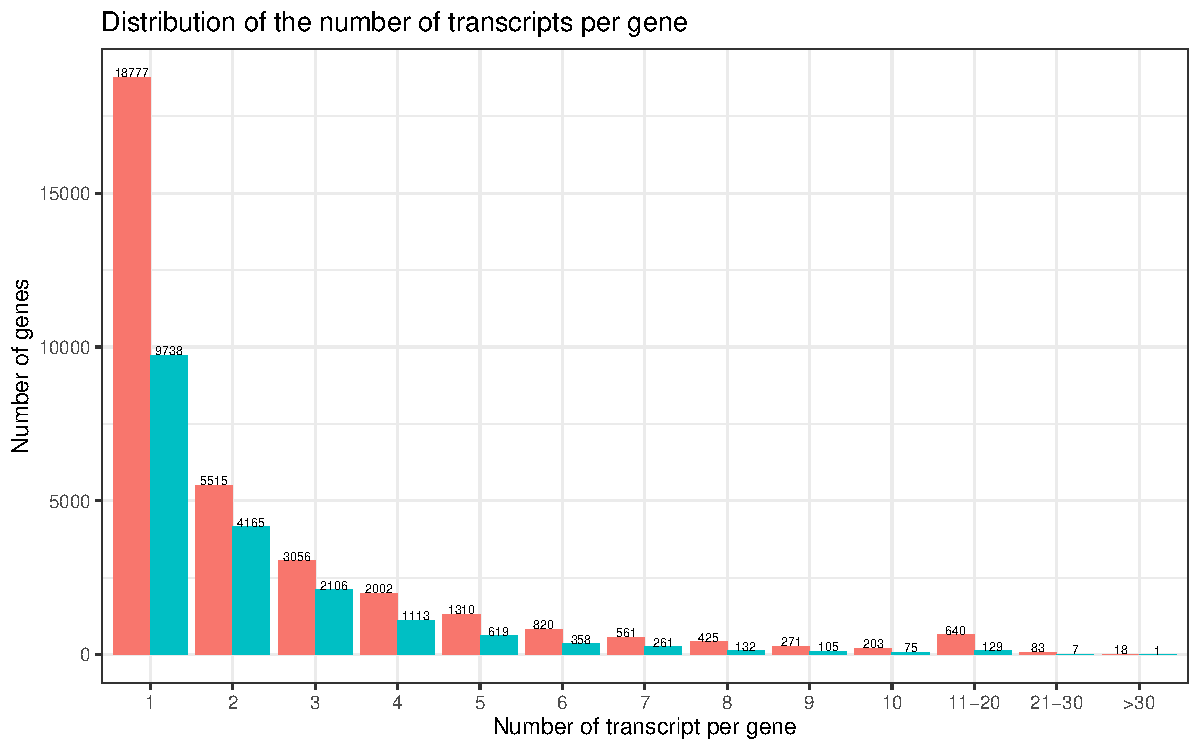
\includegraphics[width=16.67in]{X2025.01.13.16.34.12.j145/figure/Distribution of the number of transcripts per gene}

Figure: Distribution of the number of transcripts per gene. Low
expressed transcripts and genes are filtered.

\subsubsection{Number of 3D genes and
transcripts}\label{number-of-3d-genes-and-transcripts}

\begin{longtable}[]{@{}ll@{}}
\caption{RNA-seq sample information before and after data
pre-processing.}\tabularnewline
\toprule
Description & Number\tabularnewline
\midrule
\endfirsthead
\toprule
Description & Number\tabularnewline
\midrule
\endhead
Raw transcripts & 81620\tabularnewline
Raw genes & 33681\tabularnewline
Samples & 60\tabularnewline
Samples after merging seq-reps & 60\tabularnewline
Condition of interest & 20\tabularnewline
CPM cut-off & 1\tabularnewline
Min samples to CPM cut-off & 3\tabularnewline
Expressed transcripts & 40568\tabularnewline
Expressed genes & 18809\tabularnewline
\bottomrule
\end{longtable}

\begin{longtable}[]{@{}lllll@{}}
\caption{Number of DE/DAS genes and DE/DTU transcripts in different
contrast groups.}\tabularnewline
\toprule
contrast & DE genes & DAS genes & DE transcripts & DTU
transcripts\tabularnewline
\midrule
\endfirsthead
\toprule
contrast & DE genes & DAS genes & DE transcripts & DTU
transcripts\tabularnewline
\midrule
\endhead
SETI\_WT.P-SETI\_WT.mock & 7212 & 110 & 8094 & 143\tabularnewline
SETI\_WT.E-SETI\_WT.mock & 2159 & 66 & 2424 & 88\tabularnewline
SETI\_WT.PE-SETI\_WT.mock & 5938 & 81 & 6312 & 114\tabularnewline
SETI\_e.P-SETI\_e.mock & 9158 & 196 & 11069 & 243\tabularnewline
SETI\_e.E-SETI\_e.mock & 0 & 25 & 4 & 16\tabularnewline
SETI\_e.PE-SETI\_e.mock & 8962 & 194 & 10724 & 281\tabularnewline
SETI\_p.P-SETI\_p.mock & 8851 & 156 & 10368 & 212\tabularnewline
SETI\_p.E-SETI\_p.mock & 1374 & 29 & 1304 & 38\tabularnewline
SETI\_p.PE-SETI\_p.mock & 8960 & 172 & 10497 & 244\tabularnewline
SETI\_s.P-SETI\_s.mock & 8961 & 171 & 10577 & 200\tabularnewline
SETI\_s.E-SETI\_s.mock & 2959 & 88 & 3089 & 126\tabularnewline
SETI\_s.PE-SETI\_s.mock & 8349 & 154 & 9629 & 240\tabularnewline
SETI\_ps.P-SETI\_ps.mock & 8243 & 153 & 9533 & 189\tabularnewline
SETI\_ps.E-SETI\_ps.mock & 0 & 19 & 2 & 14\tabularnewline
SETI\_ps.PE-SETI\_ps.mock & 8771 & 155 & 10242 & 217\tabularnewline
\bottomrule
\end{longtable}

\begin{longtable}[]{@{}llll@{}}
\caption{Number of DE vs DAS genes.}\tabularnewline
\toprule
Contrast & DEonly & DE\&DAS & DASonly\tabularnewline
\midrule
\endfirsthead
\toprule
Contrast & DEonly & DE\&DAS & DASonly\tabularnewline
\midrule
\endhead
SETI\_WT.P-SETI\_WT.mock & 7147 & 65 & 45\tabularnewline
SETI\_WT.E-SETI\_WT.mock & 2138 & 21 & 45\tabularnewline
SETI\_WT.PE-SETI\_WT.mock & 5899 & 39 & 42\tabularnewline
SETI\_e.P-SETI\_e.mock & 9035 & 123 & 73\tabularnewline
SETI\_e.E-SETI\_e.mock & 0 & 0 & 25\tabularnewline
SETI\_e.PE-SETI\_e.mock & 8842 & 120 & 74\tabularnewline
SETI\_p.P-SETI\_p.mock & 8753 & 98 & 58\tabularnewline
SETI\_p.E-SETI\_p.mock & 1370 & 4 & 25\tabularnewline
SETI\_p.PE-SETI\_p.mock & 8851 & 109 & 63\tabularnewline
SETI\_s.P-SETI\_s.mock & 8854 & 107 & 64\tabularnewline
SETI\_s.E-SETI\_s.mock & 2929 & 30 & 58\tabularnewline
SETI\_s.PE-SETI\_s.mock & 8259 & 90 & 64\tabularnewline
SETI\_ps.P-SETI\_ps.mock & 8151 & 92 & 61\tabularnewline
SETI\_ps.E-SETI\_ps.mock & 0 & 0 & 19\tabularnewline
SETI\_ps.PE-SETI\_ps.mock & 8666 & 105 & 50\tabularnewline
\bottomrule
\end{longtable}

\begin{longtable}[]{@{}llll@{}}
\caption{Number of DE vs DTU transcripts.}\tabularnewline
\toprule
Contrast & DEonly & DE\&DTU & DTUonly\tabularnewline
\midrule
\endfirsthead
\toprule
Contrast & DEonly & DE\&DTU & DTUonly\tabularnewline
\midrule
\endhead
SETI\_WT.P-SETI\_WT.mock & 8003 & 91 & 52\tabularnewline
SETI\_WT.E-SETI\_WT.mock & 2381 & 43 & 45\tabularnewline
SETI\_WT.PE-SETI\_WT.mock & 6240 & 72 & 42\tabularnewline
SETI\_e.P-SETI\_e.mock & 10903 & 166 & 77\tabularnewline
SETI\_e.E-SETI\_e.mock & 2 & 2 & 14\tabularnewline
SETI\_e.PE-SETI\_e.mock & 10539 & 185 & 96\tabularnewline
SETI\_p.P-SETI\_p.mock & 10233 & 135 & 77\tabularnewline
SETI\_p.E-SETI\_p.mock & 1289 & 15 & 23\tabularnewline
SETI\_p.PE-SETI\_p.mock & 10352 & 145 & 99\tabularnewline
SETI\_s.P-SETI\_s.mock & 10441 & 136 & 64\tabularnewline
SETI\_s.E-SETI\_s.mock & 3024 & 65 & 61\tabularnewline
SETI\_s.PE-SETI\_s.mock & 9481 & 148 & 92\tabularnewline
SETI\_ps.P-SETI\_ps.mock & 9417 & 116 & 73\tabularnewline
SETI\_ps.E-SETI\_ps.mock & 2 & 0 & 14\tabularnewline
SETI\_ps.PE-SETI\_ps.mock & 10105 & 137 & 80\tabularnewline
\bottomrule
\end{longtable}

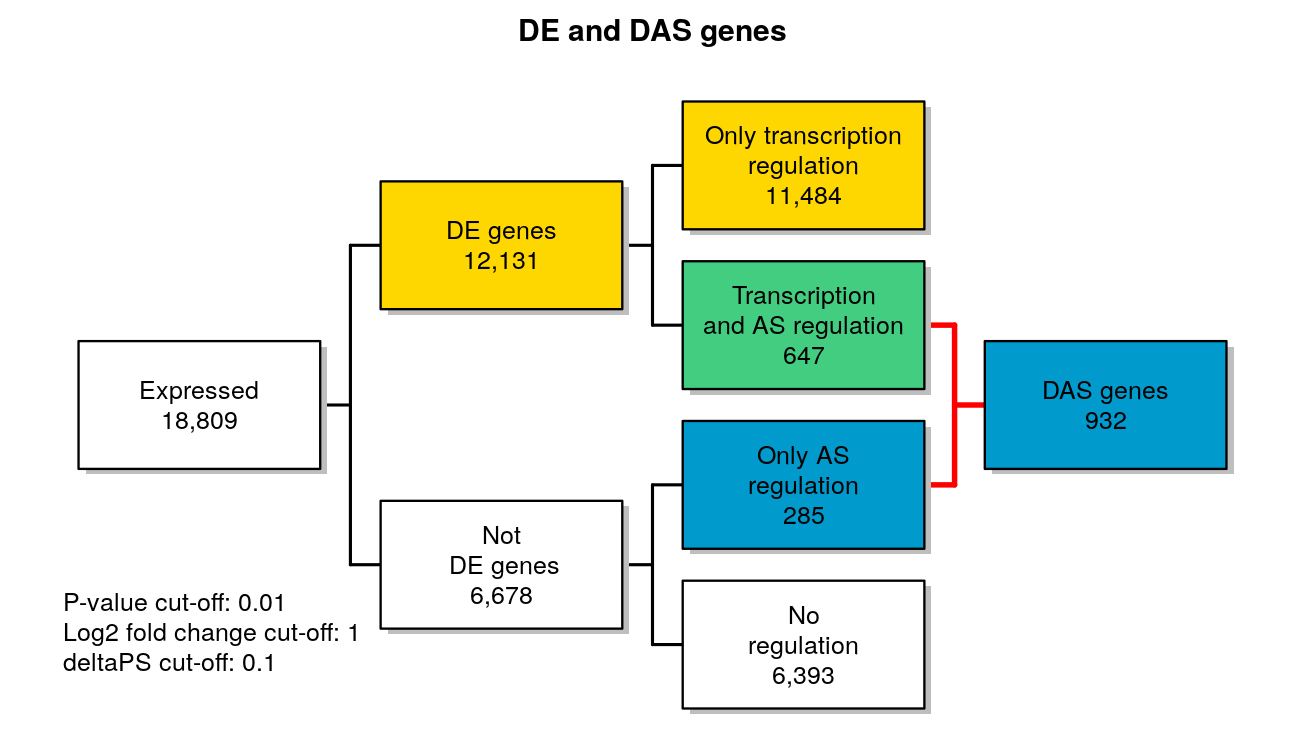
\includegraphics[width=18.12in]{X2025.01.13.16.34.12.j145/figure/Union set DE genes vs DAS genes}

Figure: Number of genes regulated only by transcription (DE), only by
alternative splicing (DAS) and by both transcription and alternative
splicing (DE+DAS).

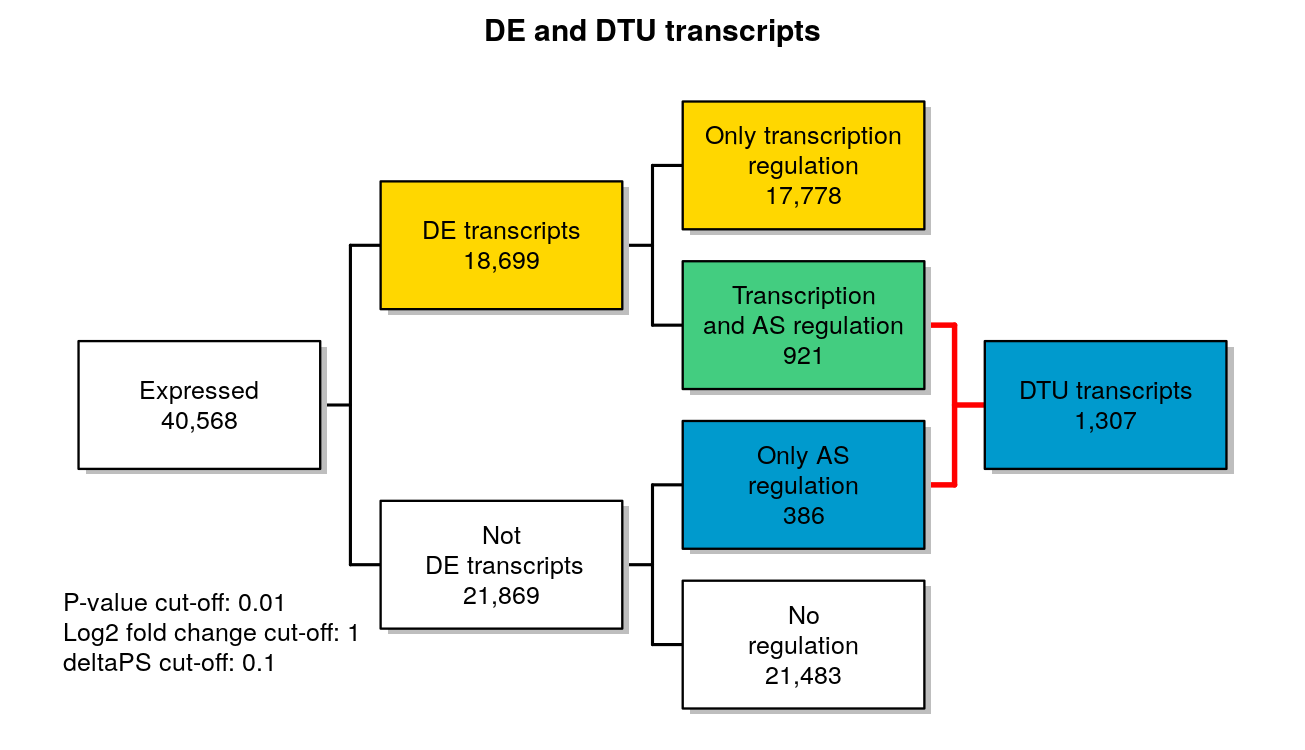
\includegraphics[width=18.12in]{X2025.01.13.16.34.12.j145/figure/Union set DE transcripts vs DTU transcripts}

Figure: Number of transcripts regulated only by transcription (DE), only
by alternative splicing (DAS) and by both transcription and alternative
splicing (DE+DAS).

\begin{verbatim}
## Results are not found.
\end{verbatim}

\subsubsection{Up- and down-regulation}\label{up--and-down-regulation}

Figure: Number of up and down regulated genes, DAS genes, DE transcripts
and DTU transcripts. The numbers are calculated based on positive or
negative signs on the \(L_2FCs\) of DE/DAS genes and DE/DTU transcripts.

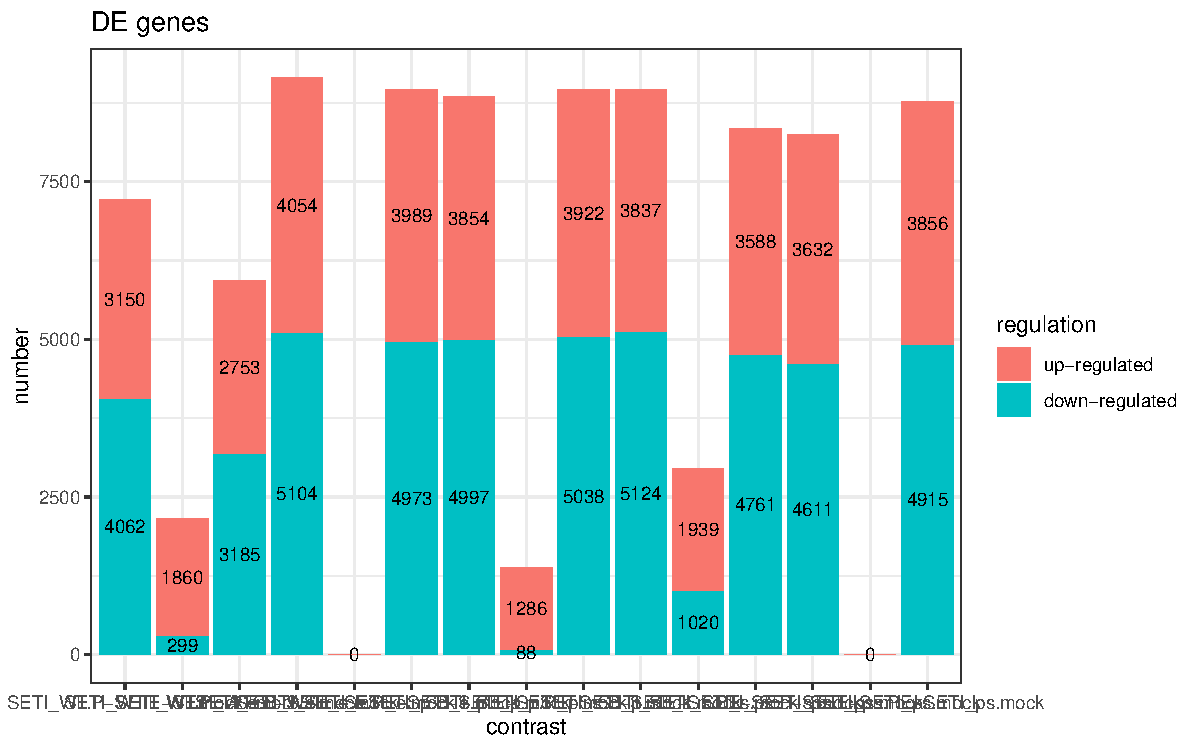
\includegraphics[width=16.67in]{X2025.01.13.16.34.12.j145/figure/DE genes up and down regulation numbers}

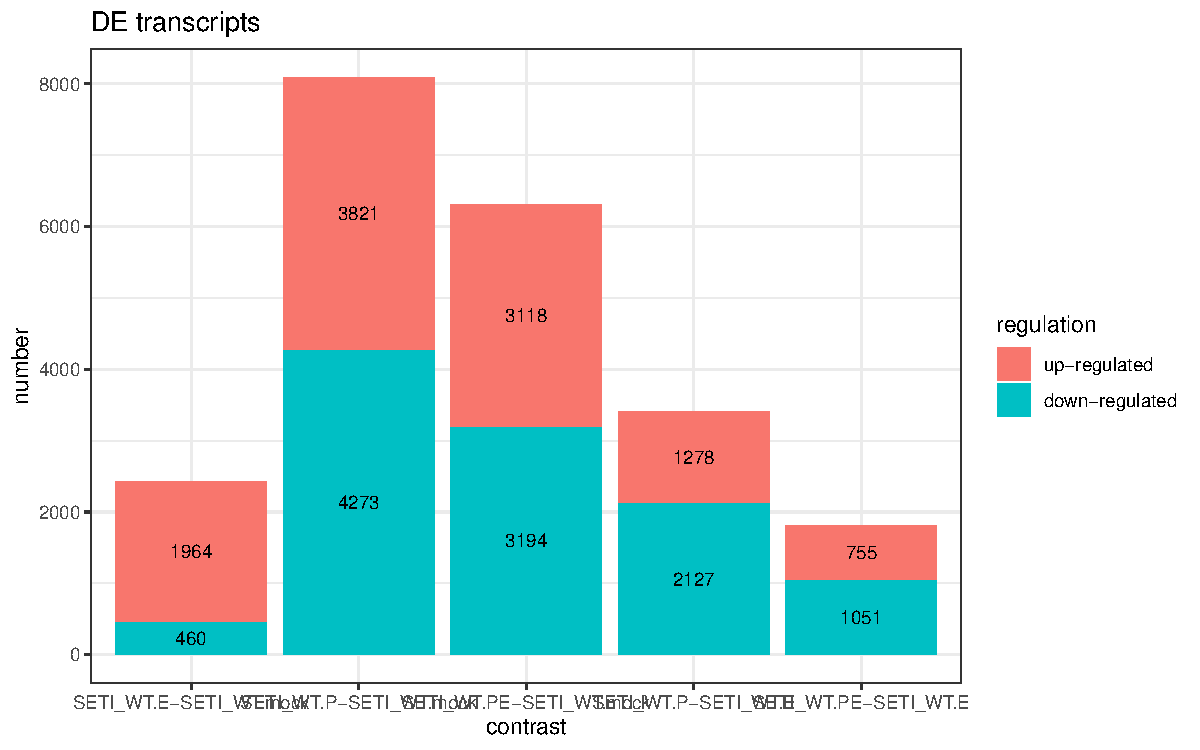
\includegraphics[width=16.67in]{X2025.01.13.16.34.12.j145/figure/DE transcripts up and down regulation numbers}

\subsubsection{Volcano plot}\label{volcano-plot}

Figure: Volcano plot. The low expressed genes and transcripts were
filtered. DE genes: log2FC vs -log10(FDR) at gene level; DAS genes:
maximum \(\Delta PS\) of transcript in a gene vs -log10(FDR) at gene
level; DE transcripts: log2FC vs -log10(FDR) at gene level at transcript
level and DTU transcripts: \(\Delta PS\) vs -log10(FDR) at transcript
level.

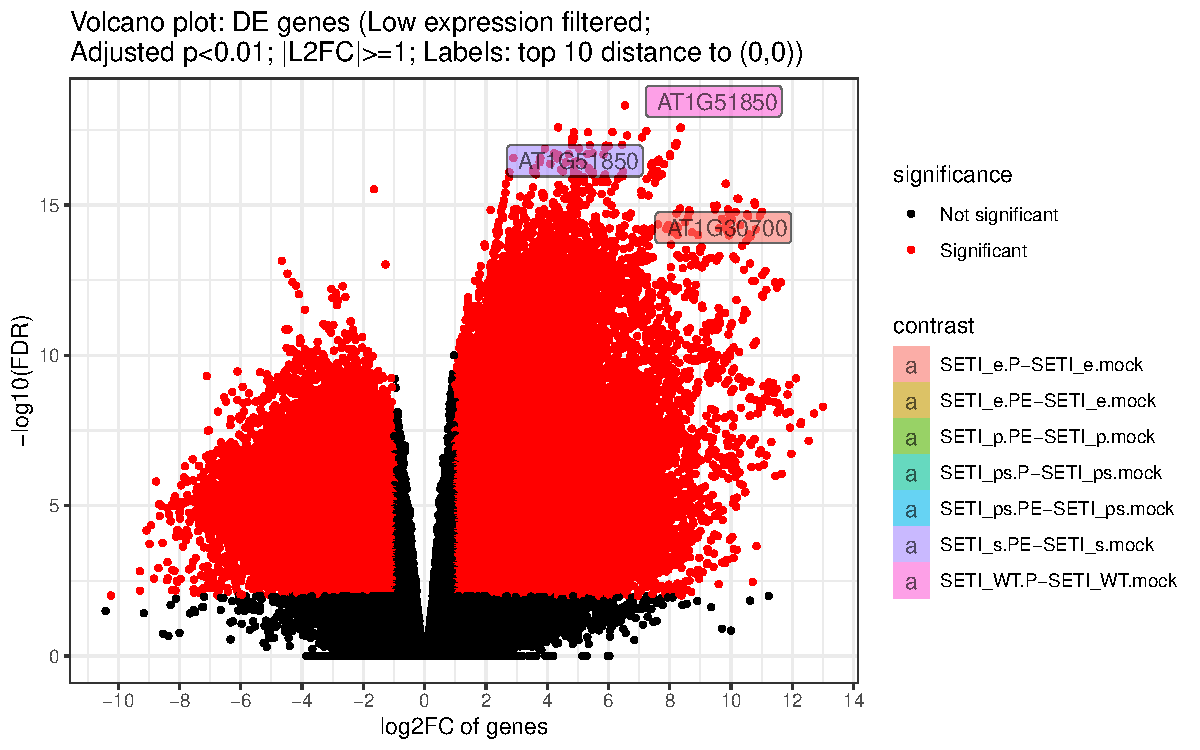
\includegraphics[width=16.67in]{X2025.01.13.16.34.12.j145/figure/DE genes volcano plot}

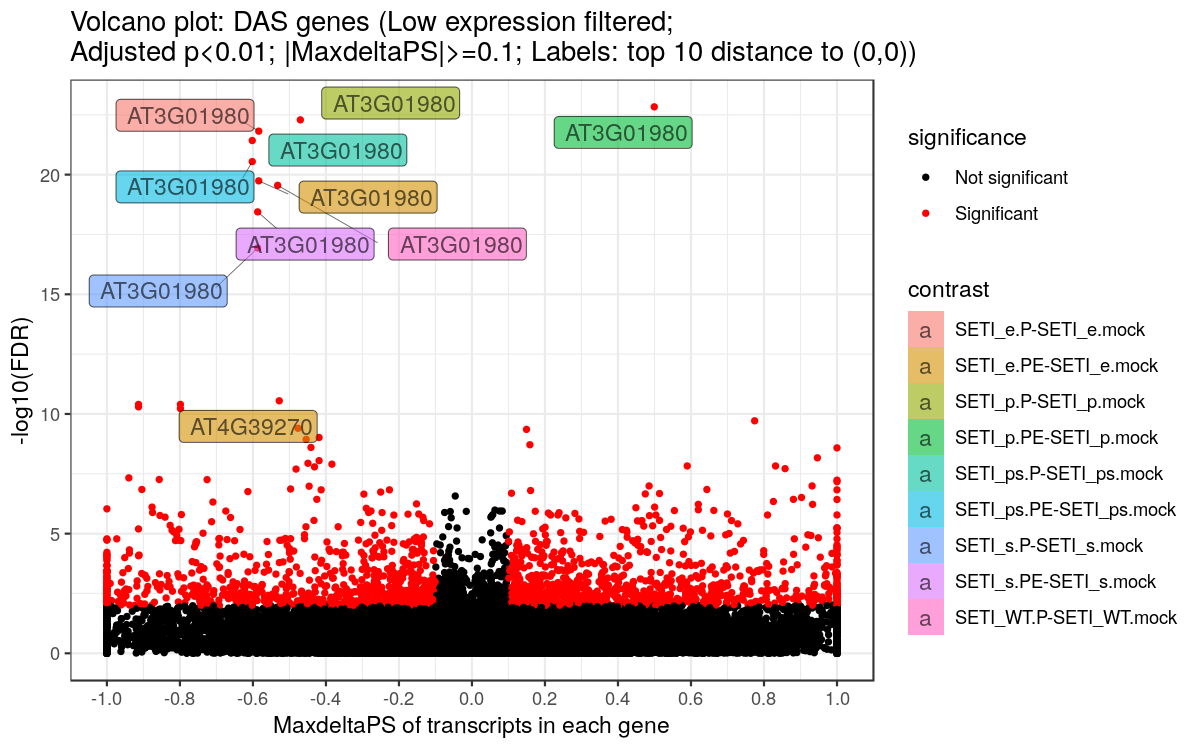
\includegraphics[width=16.67in]{X2025.01.13.16.34.12.j145/figure/DAS genes volcano plot}

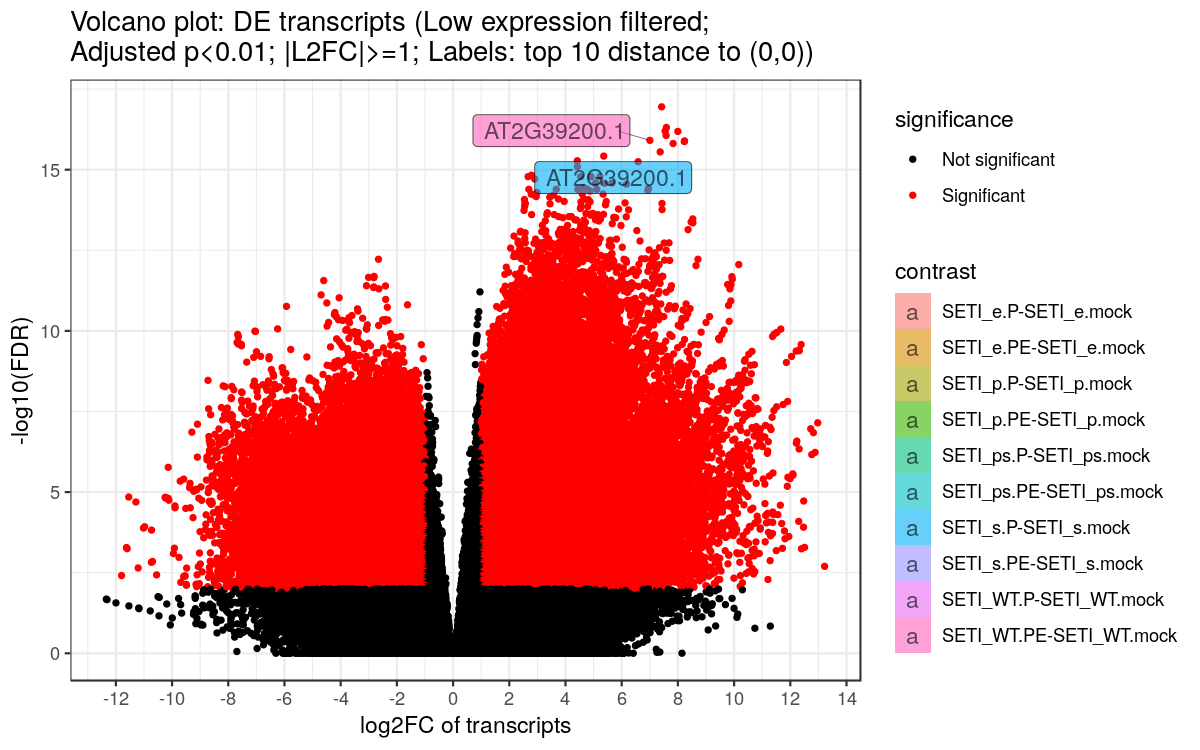
\includegraphics[width=16.67in]{X2025.01.13.16.34.12.j145/figure/DE transcripts volcano plot}

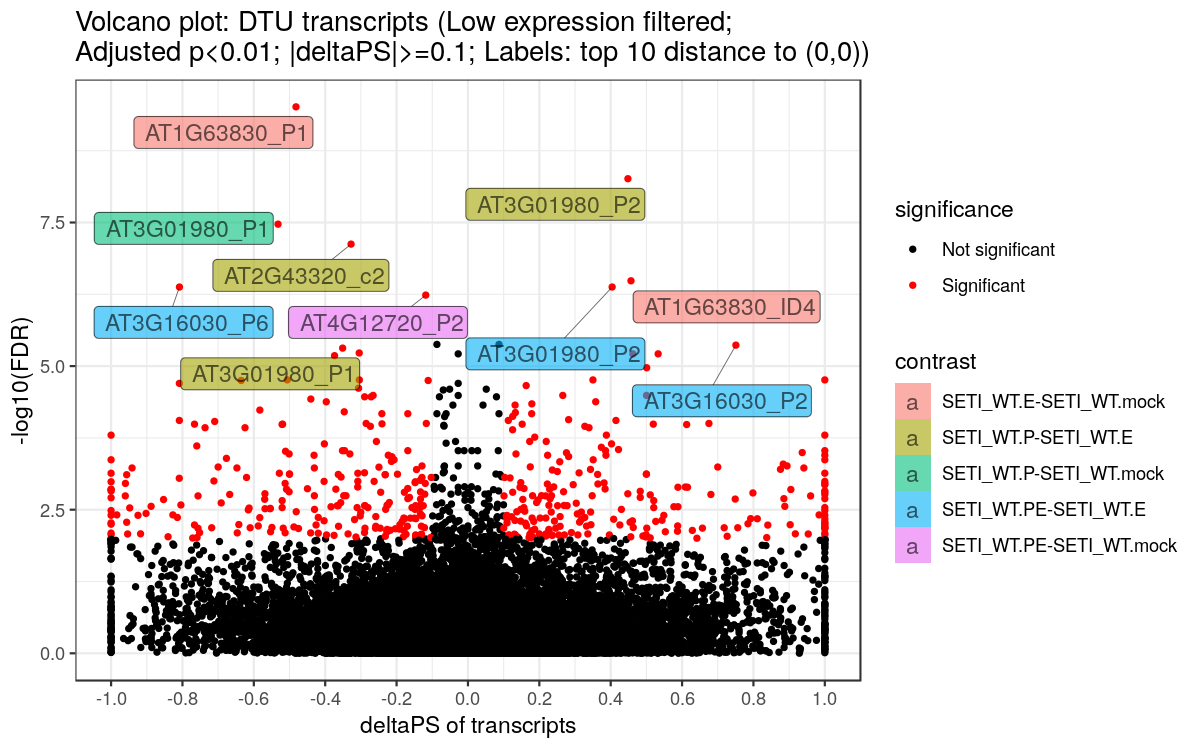
\includegraphics[width=16.67in]{X2025.01.13.16.34.12.j145/figure/DTU transcripts volcano plot}

\subsubsection{Heatmap}\label{heatmap}

Hierarchical clustering was used to partition the DE genes into 10
clusters with euclidean distance and ward.D clustering algorithm
(Saracli et al., 2013). ComplexHeatmap R package version 1.20.0 was used
to make the heat-maps.

Figure: Heatmap of DE genes, including DE only and DE+DAS genes.

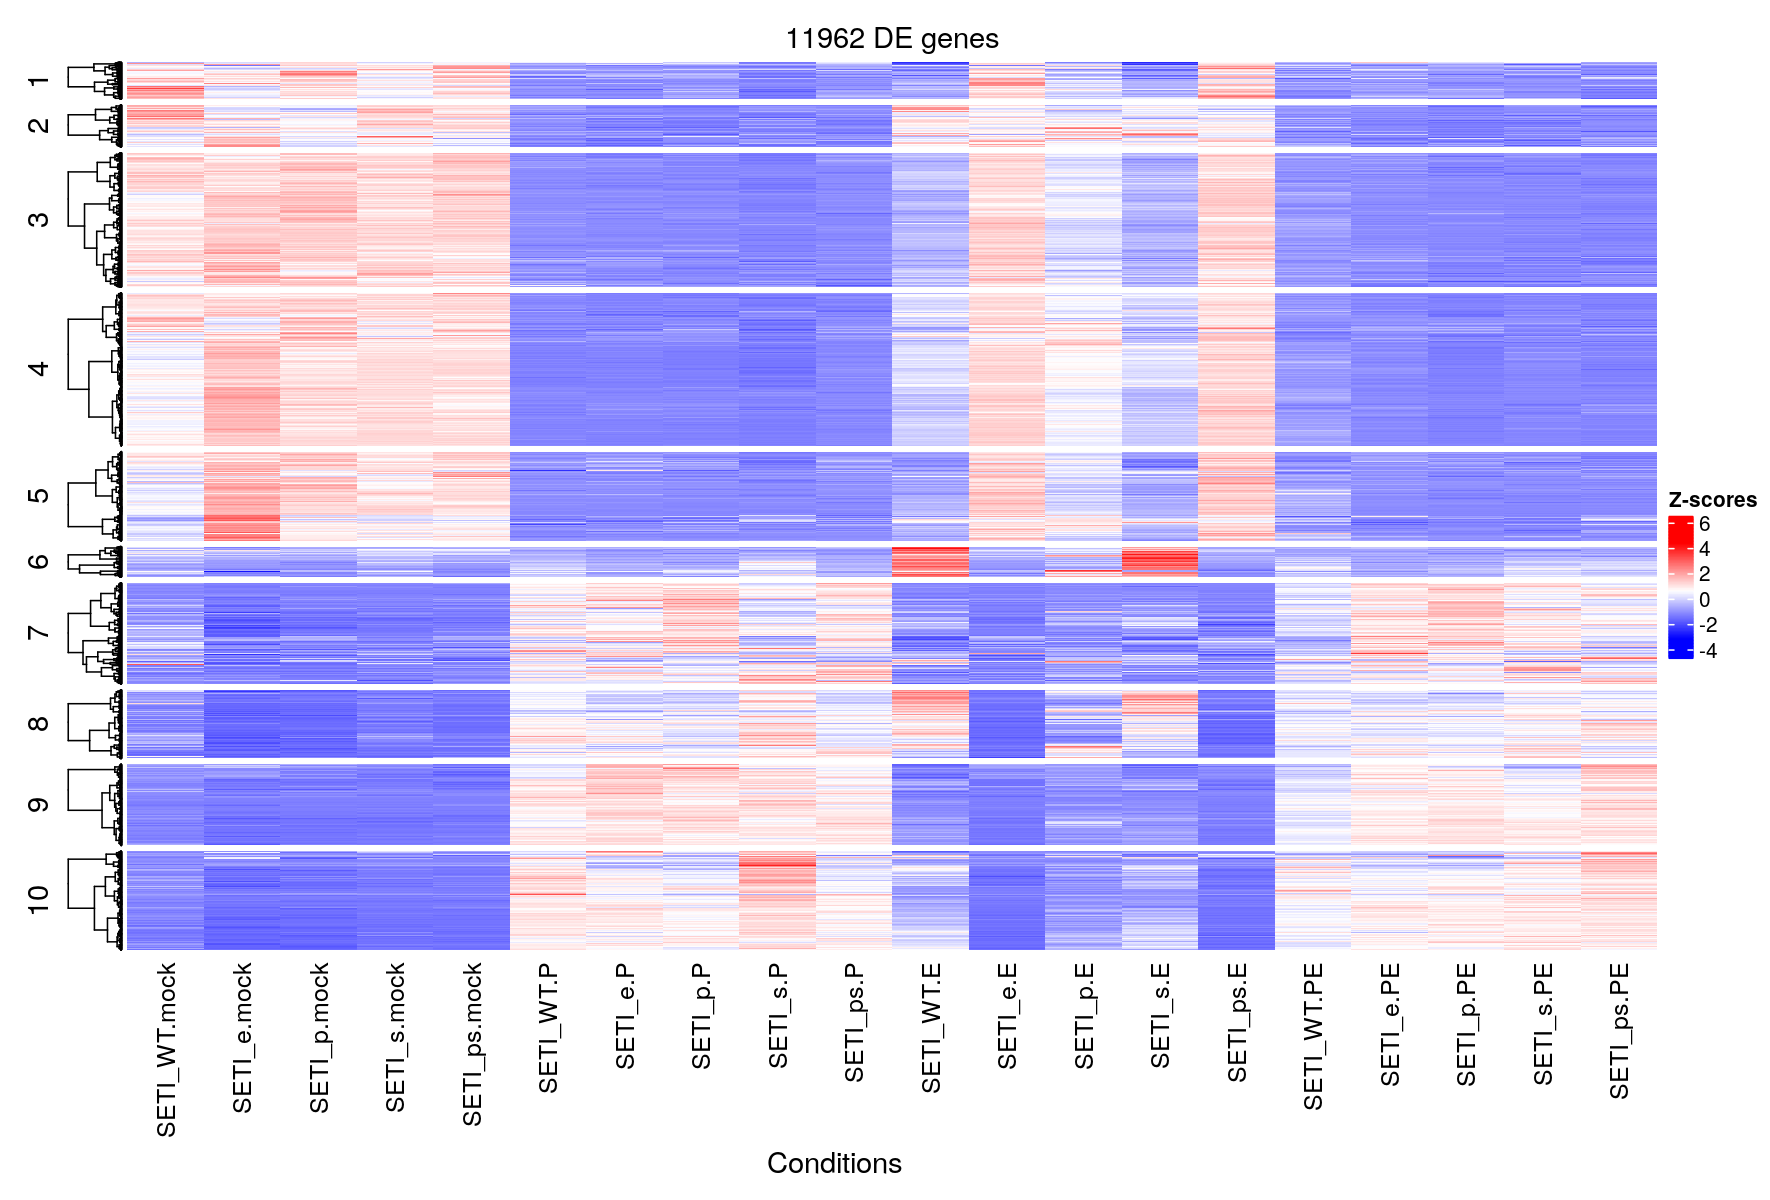
\includegraphics[width=24.58in]{X2025.01.13.16.34.12.j145/figure/Heatmap DE genes}

Figure: Heatmap of DE+DAS genes. The genes of DAS only were removed
since they only had significant alternative splicing changes, but did
not have significant expression changes.

\begin{verbatim}
## Plot is not found in the figure folder
\end{verbatim}

Figure: Heatmap of DE transcripts, including DE only and DE+DTU
transcripts.

\begin{verbatim}
## Plot is not found in the figure folder
\end{verbatim}

Figure: Heatmap of DE+DTU transcripts.DTU only transcripts were removed
since they only had significant alternative splicing changes, but did
not have significant expression changes.

\begin{verbatim}
## Plot is not found in the figure folder
\end{verbatim}

\subsubsection{GO annotation plot}\label{go-annotation-plot}

Figure: Significant GO enriched terms of DE genes.

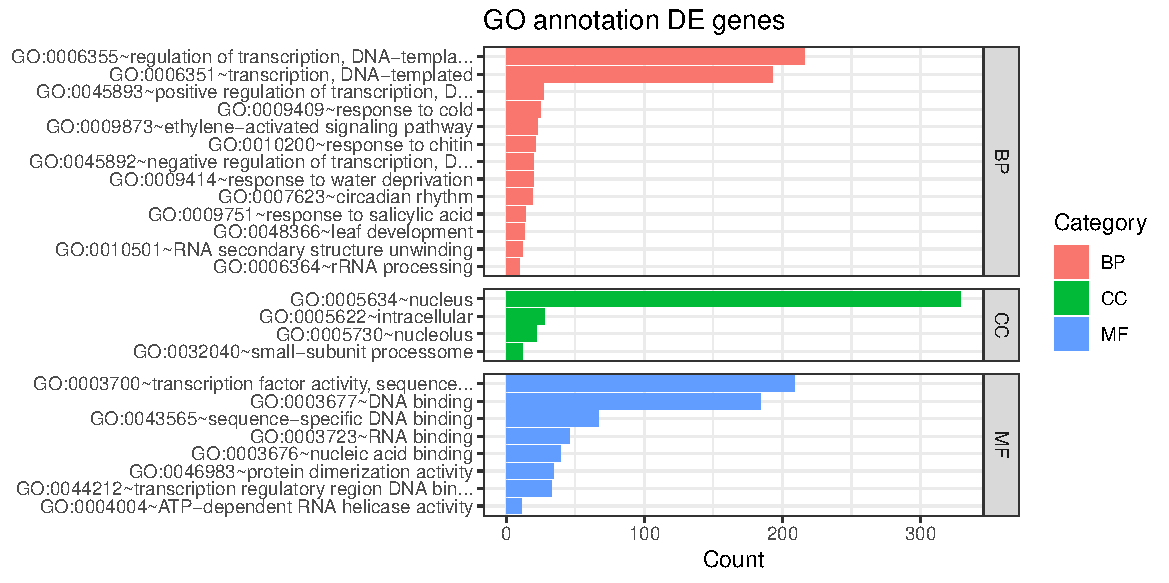
\includegraphics[width=16.25in]{X2025.01.13.16.34.12.j145/figure/DE genes GO annotation plot}

Figure: Significant GO enriched terms of DAS genes.

\begin{verbatim}
## Plot is not found in the figure folder
\end{verbatim}

\subsubsection{Significant isoform
switches}\label{significant-isoform-switches}

Figure: Significant isoform switches between transcript isoforms.

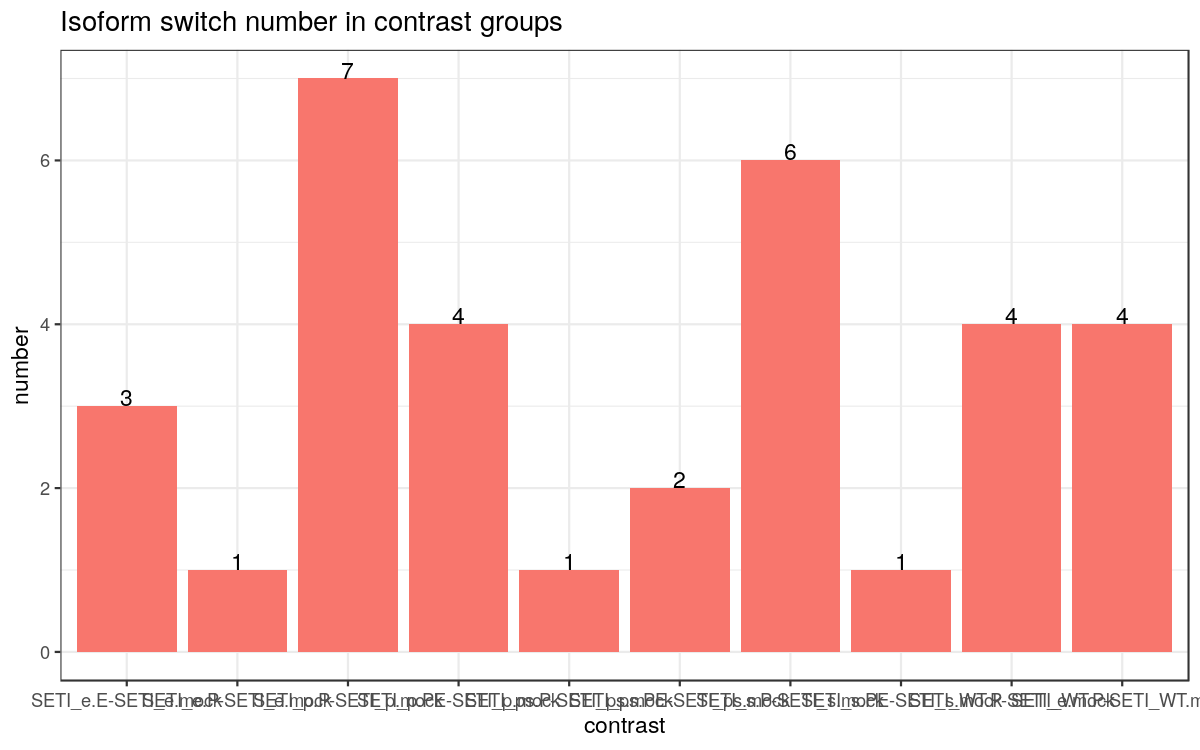
\includegraphics[width=16.67in]{X2025.01.13.16.34.12.j145/figure/Isoform switch number}

\subsection{Supplementary figures}\label{supplementary-figures}

\subsubsection{Mean-variance trend plot}\label{mean-variance-trend-plot}

The cut-offs to filter the transcripts were determined by the
mean-variance trend plots (Law et al. 2014).

\begin{itemize}
\tightlist
\item
  An expressed transcript must have \(\geq\) 3 out of 9 samples with CPM
  \(\geq\) 1.
\item
  An expressed gene must have at least one expressed transcript.
\end{itemize}

Figure: Transcript level mean-variance trend plot

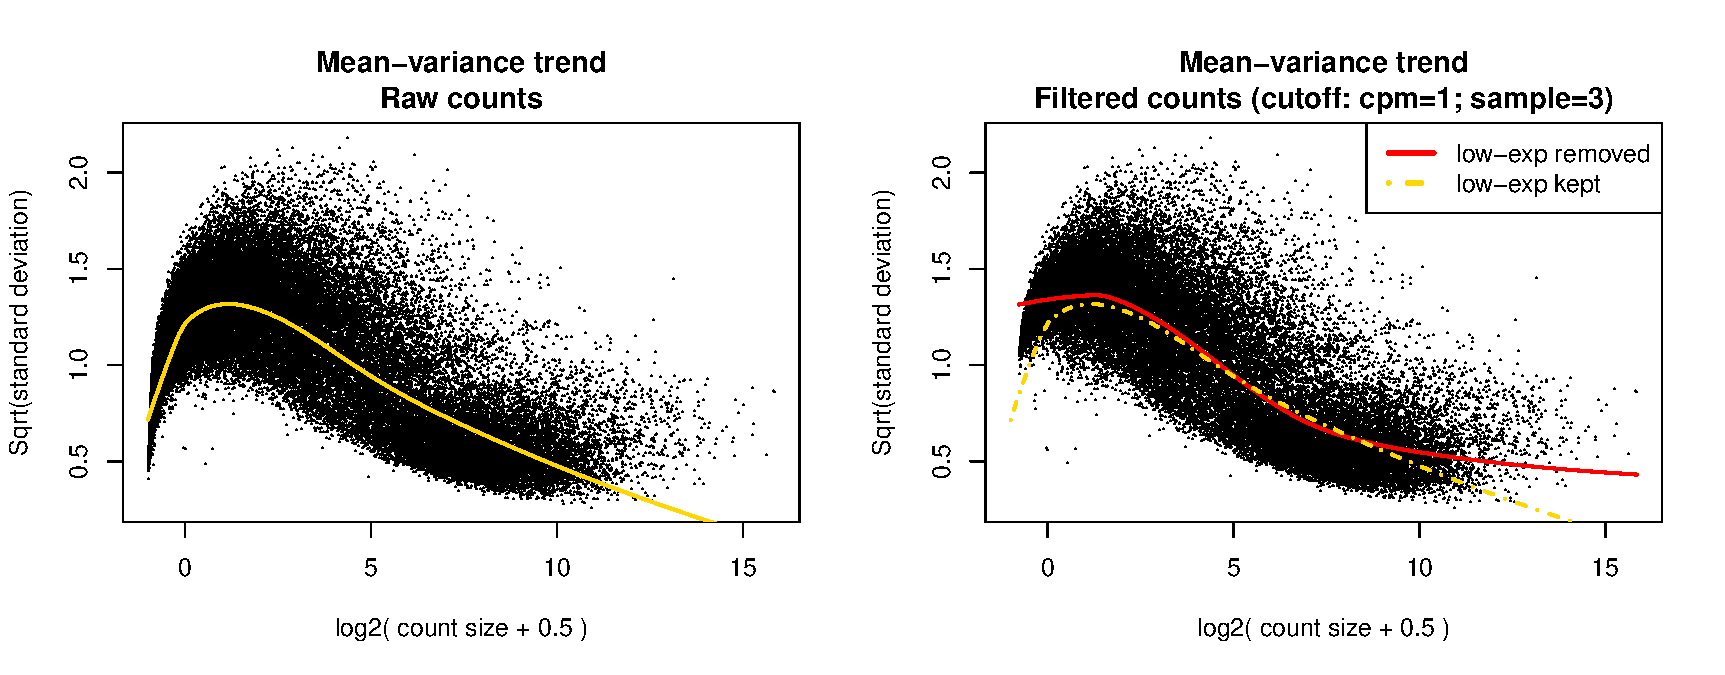
\includegraphics[width=23.96in]{X2025.01.13.16.34.12.j145/figure/Transcript mean-variance trend}

Figure: Gene level mean-variance trend plot

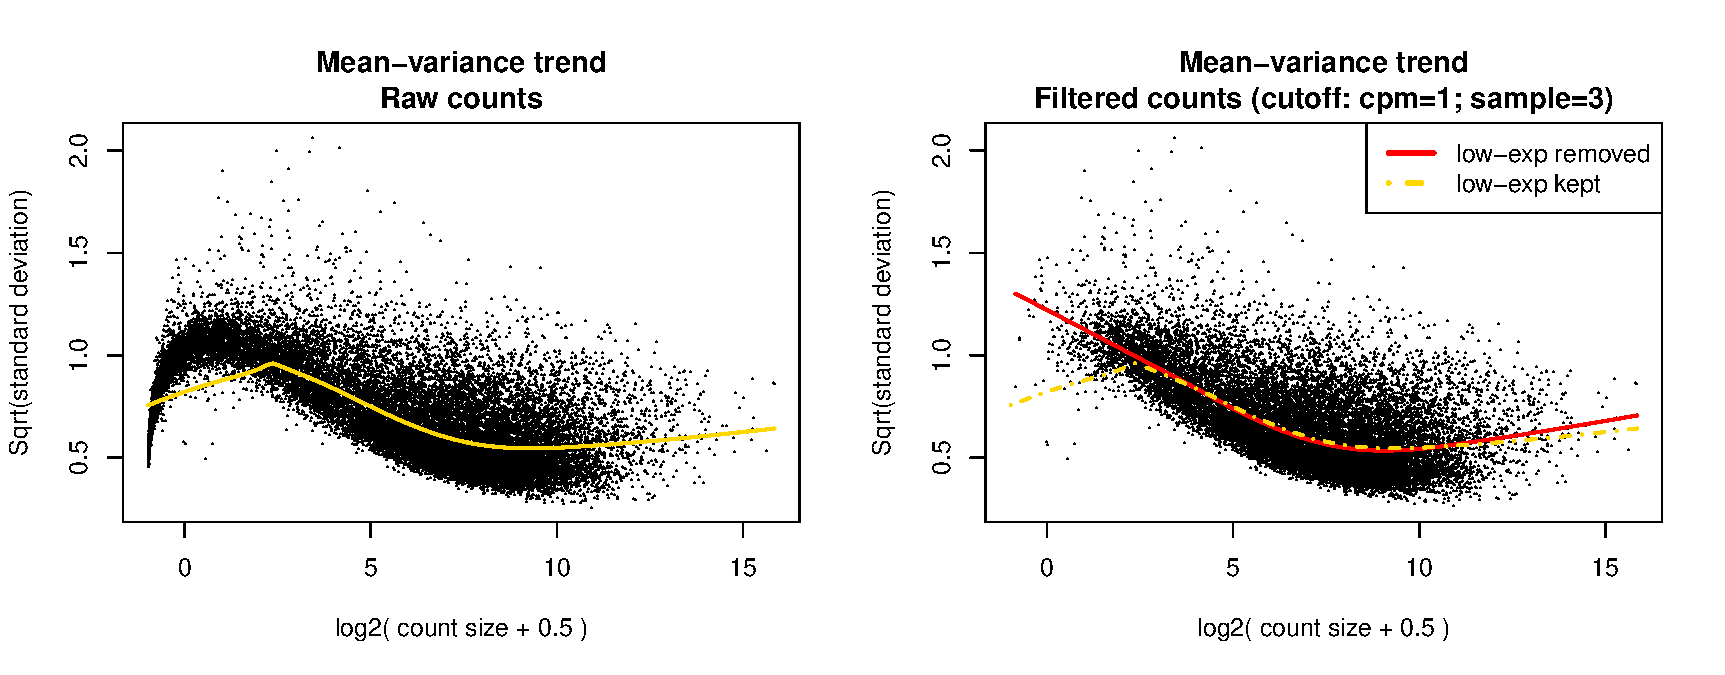
\includegraphics[width=23.96in]{X2025.01.13.16.34.12.j145/figure/Gene mean-variance trend}

\subsubsection{PCA plot of all samples}\label{pca-plot-of-all-samples}

The normalised \(log_2\)-CPM of all samples were used to make PCA plots.
The PCA plot of all samples can be found in the figure folder.

\subsubsection{Sample distribution}\label{sample-distribution}

Figure: Transcript level read counts and normalised \(log_2\)-CPM
distribution across samples.

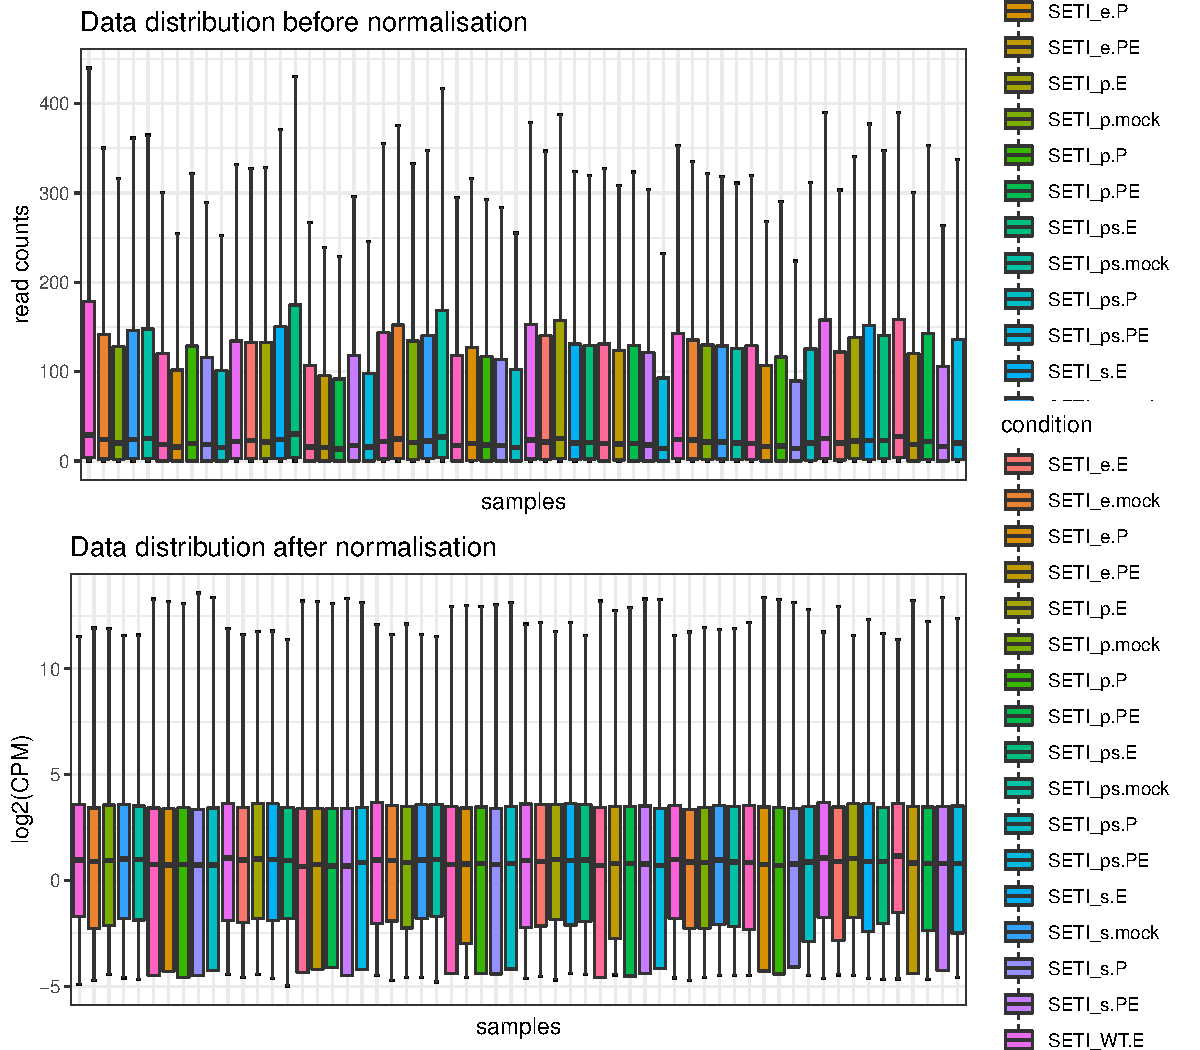
\includegraphics[width=16.67in]{X2025.01.13.16.34.12.j145/figure/Transcript expression distribution}

Figure: Gene level read counts and normalised \(log_2\)-CPM distribution
across samples.

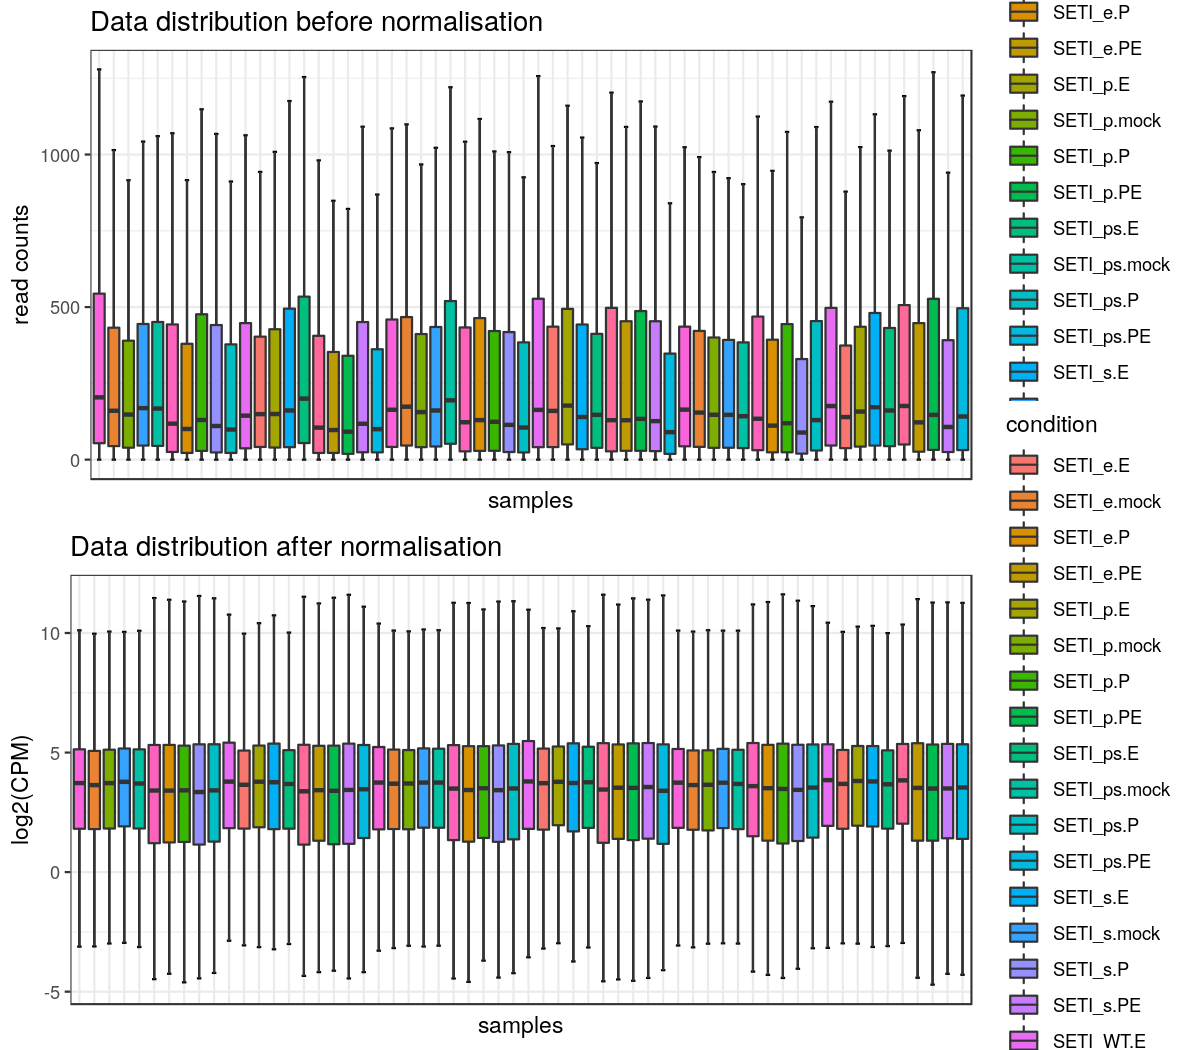
\includegraphics[width=16.67in]{X2025.01.13.16.34.12.j145/figure/Gene expression distribution}

\subsubsection{Venn diagrams}\label{venn-diagrams}

Venn diagrams to compare significant DE genes, DAS genes, DE transcript
and DTU transcripts in different contrast groups can be found in figure
folder.

\subsection{Supplementary materials}\label{supplementary-materials}

\subsubsection{Files in report folder}\label{files-in-report-folder}

Reports are saved in report folder.

\begin{longtable}[]{@{}ll@{}}
\toprule
File name & Description\tabularnewline
\midrule
\endhead
3D\_report.pdf/html/doc & Report of 3D analysis in pdf, html and doc
format\tabularnewline
\bottomrule
\end{longtable}

\subsubsection{Files in figure folder}\label{files-in-figure-folder}

\begin{longtable}[]{@{}ll@{}}
\toprule
\begin{minipage}[b]{0.51\columnwidth}\raggedright\strut
File.names\strut
\end{minipage} & \begin{minipage}[b]{0.43\columnwidth}\raggedright\strut
Description\strut
\end{minipage}\tabularnewline
\midrule
\endhead
\begin{minipage}[t]{0.51\columnwidth}\raggedright\strut
DAS genes GO annotation plot.png/.pdf\strut
\end{minipage} & \begin{minipage}[t]{0.43\columnwidth}\raggedright\strut
DAS genes GO annotation plot\strut
\end{minipage}\tabularnewline
\begin{minipage}[t]{0.51\columnwidth}\raggedright\strut
DAS genes updown regulation numbers.png/.pdf\strut
\end{minipage} & \begin{minipage}[t]{0.43\columnwidth}\raggedright\strut
DAS genes up-down regulation numbers\strut
\end{minipage}\tabularnewline
\begin{minipage}[t]{0.51\columnwidth}\raggedright\strut
DAS genes volcano plot.png/.pdf\strut
\end{minipage} & \begin{minipage}[t]{0.43\columnwidth}\raggedright\strut
DAS genes volcano plot\strut
\end{minipage}\tabularnewline
\begin{minipage}[t]{0.51\columnwidth}\raggedright\strut
DE genes GO annotation plot.png/.pdf\strut
\end{minipage} & \begin{minipage}[t]{0.43\columnwidth}\raggedright\strut
DE genes GO annotation plot\strut
\end{minipage}\tabularnewline
\begin{minipage}[t]{0.51\columnwidth}\raggedright\strut
DE genes updown regulation numbers.png/.pdf\strut
\end{minipage} & \begin{minipage}[t]{0.43\columnwidth}\raggedright\strut
DE genes up-down regulation numbers\strut
\end{minipage}\tabularnewline
\begin{minipage}[t]{0.51\columnwidth}\raggedright\strut
DE genes volcano plot.png/.pdf\strut
\end{minipage} & \begin{minipage}[t]{0.43\columnwidth}\raggedright\strut
DE genes volcano plot\strut
\end{minipage}\tabularnewline
\begin{minipage}[t]{0.51\columnwidth}\raggedright\strut
DE transcripts updown regulation numbers.png/.pdf\strut
\end{minipage} & \begin{minipage}[t]{0.43\columnwidth}\raggedright\strut
DE transcripts up-down regulation numbers\strut
\end{minipage}\tabularnewline
\begin{minipage}[t]{0.51\columnwidth}\raggedright\strut
DE transcripts volcano plot.png/.pdf\strut
\end{minipage} & \begin{minipage}[t]{0.43\columnwidth}\raggedright\strut
DE transcripts volcano plot\strut
\end{minipage}\tabularnewline
\begin{minipage}[t]{0.51\columnwidth}\raggedright\strut
DTU transcripts updown regulation numbers.png/.pdf\strut
\end{minipage} & \begin{minipage}[t]{0.43\columnwidth}\raggedright\strut
DTU transcripts up-down regulation numbers\strut
\end{minipage}\tabularnewline
\begin{minipage}[t]{0.51\columnwidth}\raggedright\strut
DTU transcripts volcano plot.png/.pdf\strut
\end{minipage} & \begin{minipage}[t]{0.43\columnwidth}\raggedright\strut
DTU transcripts volcano plot\strut
\end{minipage}\tabularnewline
\begin{minipage}[t]{0.51\columnwidth}\raggedright\strut
Gene data distribution.png/.pdf\strut
\end{minipage} & \begin{minipage}[t]{0.43\columnwidth}\raggedright\strut
Gene data distribution\strut
\end{minipage}\tabularnewline
\begin{minipage}[t]{0.51\columnwidth}\raggedright\strut
Gene mean-variance trend.png/.pdf\strut
\end{minipage} & \begin{minipage}[t]{0.43\columnwidth}\raggedright\strut
Gene mean-variance trend\strut
\end{minipage}\tabularnewline
\begin{minipage}[t]{0.51\columnwidth}\raggedright\strut
Gene PCA Average expression.png/.pdf\strut
\end{minipage} & \begin{minipage}[t]{0.43\columnwidth}\raggedright\strut
Gene PCA Average expression\strut
\end{minipage}\tabularnewline
\begin{minipage}[t]{0.51\columnwidth}\raggedright\strut
Gene PCA batch effect removed Bio-reps.png/.pdf\strut
\end{minipage} & \begin{minipage}[t]{0.43\columnwidth}\raggedright\strut
Gene PCA batch effect removed Bio-reps\strut
\end{minipage}\tabularnewline
\begin{minipage}[t]{0.51\columnwidth}\raggedright\strut
Gene PCA Bio-reps.png/.pdf\strut
\end{minipage} & \begin{minipage}[t]{0.43\columnwidth}\raggedright\strut
Gene PCA Bio-reps\strut
\end{minipage}\tabularnewline
\begin{minipage}[t]{0.51\columnwidth}\raggedright\strut
Heatmap DAS genes.png/.pdf\strut
\end{minipage} & \begin{minipage}[t]{0.43\columnwidth}\raggedright\strut
Heatmap of DE+DAS genes\strut
\end{minipage}\tabularnewline
\begin{minipage}[t]{0.51\columnwidth}\raggedright\strut
Heatmap DE genes.png/.pdf\strut
\end{minipage} & \begin{minipage}[t]{0.43\columnwidth}\raggedright\strut
Heatmap of DE genes\strut
\end{minipage}\tabularnewline
\begin{minipage}[t]{0.51\columnwidth}\raggedright\strut
Heatmap DE transcripts.png/.pdf\strut
\end{minipage} & \begin{minipage}[t]{0.43\columnwidth}\raggedright\strut
Heatmap of DE transcripts\strut
\end{minipage}\tabularnewline
\begin{minipage}[t]{0.51\columnwidth}\raggedright\strut
Heatmap DTU transcripts.png/.pdf\strut
\end{minipage} & \begin{minipage}[t]{0.43\columnwidth}\raggedright\strut
Heatmap of DE+DTU transcripts\strut
\end{minipage}\tabularnewline
\begin{minipage}[t]{0.51\columnwidth}\raggedright\strut
Transcript data distribution.png/.pdf\strut
\end{minipage} & \begin{minipage}[t]{0.43\columnwidth}\raggedright\strut
Transcript data distribution\strut
\end{minipage}\tabularnewline
\begin{minipage}[t]{0.51\columnwidth}\raggedright\strut
Transcript mean-variance trend.png/.pdf\strut
\end{minipage} & \begin{minipage}[t]{0.43\columnwidth}\raggedright\strut
Transcript mean-variance trend\strut
\end{minipage}\tabularnewline
\begin{minipage}[t]{0.51\columnwidth}\raggedright\strut
Transcript PCA Average expression.png/.pdf\strut
\end{minipage} & \begin{minipage}[t]{0.43\columnwidth}\raggedright\strut
Transcript PCA Average expression\strut
\end{minipage}\tabularnewline
\begin{minipage}[t]{0.51\columnwidth}\raggedright\strut
Transcript PCA batch effect removed Bio-reps.png/.pdf\strut
\end{minipage} & \begin{minipage}[t]{0.43\columnwidth}\raggedright\strut
Transcript PCA batch effect removed Bio-reps\strut
\end{minipage}\tabularnewline
\begin{minipage}[t]{0.51\columnwidth}\raggedright\strut
Transcript PCA Bio-reps.png/.pdf\strut
\end{minipage} & \begin{minipage}[t]{0.43\columnwidth}\raggedright\strut
Transcript PCA Bio-reps\strut
\end{minipage}\tabularnewline
\begin{minipage}[t]{0.51\columnwidth}\raggedright\strut
Union set DE genes vs DAS genes.png/.pdf\strut
\end{minipage} & \begin{minipage}[t]{0.43\columnwidth}\raggedright\strut
Flow chart -Union set DE genes vs DAS genes\strut
\end{minipage}\tabularnewline
\begin{minipage}[t]{0.51\columnwidth}\raggedright\strut
Union set DE transcripts vs DTU transcripts.png/.pdf\strut
\end{minipage} & \begin{minipage}[t]{0.43\columnwidth}\raggedright\strut
Flow chart -Union set DE transcripts vs DTU transcripts\strut
\end{minipage}\tabularnewline
\begin{minipage}[t]{0.51\columnwidth}\raggedright\strut
Isoform switch number.png/.pdf\strut
\end{minipage} & \begin{minipage}[t]{0.43\columnwidth}\raggedright\strut
Number of significant isoform switch numbers in contrast groups\strut
\end{minipage}\tabularnewline
\bottomrule
\end{longtable}

\subsubsection{Files in result folder}\label{files-in-result-folder}

Important results are saved in csv (comma delimited) files.

\begin{longtable}[]{@{}lll@{}}
\toprule
\begin{minipage}[b]{0.25\columnwidth}\raggedright\strut
csv files\strut
\end{minipage} & \begin{minipage}[b]{0.65\columnwidth}\raggedright\strut
Description\strut
\end{minipage} & \begin{minipage}[b]{0.02\columnwidth}\raggedright\strut
\strut
\end{minipage}\tabularnewline
\midrule
\endhead
\begin{minipage}[t]{0.25\columnwidth}\raggedright\strut
contrast.csv\strut
\end{minipage} & \begin{minipage}[t]{0.65\columnwidth}\raggedright\strut
Contrast groups used for 3D analysis\strut
\end{minipage} & \begin{minipage}[t]{0.02\columnwidth}\raggedright\strut
\strut
\end{minipage}\tabularnewline
\begin{minipage}[t]{0.25\columnwidth}\raggedright\strut
DDD genes and transcript lists across all contrast groups.csv\strut
\end{minipage} & \begin{minipage}[t]{0.65\columnwidth}\raggedright\strut
List of DE genes, DAS genes, DE transcripts and DTU transcripts, which
are the union sets across all contrast groups\strut
\end{minipage} & \begin{minipage}[t]{0.02\columnwidth}\raggedright\strut
\strut
\end{minipage}\tabularnewline
\begin{minipage}[t]{0.25\columnwidth}\raggedright\strut
DDD numbers.csv\strut
\end{minipage} & \begin{minipage}[t]{0.65\columnwidth}\raggedright\strut
DE/DAS/DTU genes/transcript numbers in each contrast group\strut
\end{minipage} & \begin{minipage}[t]{0.02\columnwidth}\raggedright\strut
\strut
\end{minipage}\tabularnewline
\begin{minipage}[t]{0.25\columnwidth}\raggedright\strut
DEvsDAS results.csv\strut
\end{minipage} & \begin{minipage}[t]{0.65\columnwidth}\raggedright\strut
Number of DE vs DAS genes\strut
\end{minipage} & \begin{minipage}[t]{0.02\columnwidth}\raggedright\strut
\strut
\end{minipage}\tabularnewline
\begin{minipage}[t]{0.25\columnwidth}\raggedright\strut
DEvsDTU results.csv\strut
\end{minipage} & \begin{minipage}[t]{0.65\columnwidth}\raggedright\strut
Number of DE vs DTU transcripts\strut
\end{minipage} & \begin{minipage}[t]{0.02\columnwidth}\raggedright\strut
\strut
\end{minipage}\tabularnewline
\begin{minipage}[t]{0.25\columnwidth}\raggedright\strut
Gene read counts.csv\strut
\end{minipage} & \begin{minipage}[t]{0.65\columnwidth}\raggedright\strut
Raw read counts of genes before data pre-processing\strut
\end{minipage} & \begin{minipage}[t]{0.02\columnwidth}\raggedright\strut
\strut
\end{minipage}\tabularnewline
\begin{minipage}[t]{0.25\columnwidth}\raggedright\strut
Gene TPM.csv\strut
\end{minipage} & \begin{minipage}[t]{0.65\columnwidth}\raggedright\strut
Raw TPM of genes before data pre-processing\strut
\end{minipage} & \begin{minipage}[t]{0.02\columnwidth}\raggedright\strut
\strut
\end{minipage}\tabularnewline
\begin{minipage}[t]{0.25\columnwidth}\raggedright\strut
RNAseq info.csv\strut
\end{minipage} & \begin{minipage}[t]{0.65\columnwidth}\raggedright\strut
RNA-seq data information before and after pre-processing\strut
\end{minipage} & \begin{minipage}[t]{0.02\columnwidth}\raggedright\strut
\strut
\end{minipage}\tabularnewline
\begin{minipage}[t]{0.25\columnwidth}\raggedright\strut
samples.csv\strut
\end{minipage} & \begin{minipage}[t]{0.65\columnwidth}\raggedright\strut
Sample information\strut
\end{minipage} & \begin{minipage}[t]{0.02\columnwidth}\raggedright\strut
\strut
\end{minipage}\tabularnewline
\begin{minipage}[t]{0.25\columnwidth}\raggedright\strut
Significant DE genes list and statistics.csv\strut
\end{minipage} & \begin{minipage}[t]{0.65\columnwidth}\raggedright\strut
Statistics of significant DE genes\strut
\end{minipage} & \begin{minipage}[t]{0.02\columnwidth}\raggedright\strut
\strut
\end{minipage}\tabularnewline
\begin{minipage}[t]{0.25\columnwidth}\raggedright\strut
Significant DE genes list and statistics.csv\strut
\end{minipage} & \begin{minipage}[t]{0.65\columnwidth}\raggedright\strut
Statistics of significant DAS genes\strut
\end{minipage} & \begin{minipage}[t]{0.02\columnwidth}\raggedright\strut
\strut
\end{minipage}\tabularnewline
\begin{minipage}[t]{0.25\columnwidth}\raggedright\strut
Significant DE transcripts list and statistics.csv\strut
\end{minipage} & \begin{minipage}[t]{0.65\columnwidth}\raggedright\strut
Statistics of significant DE transcripts\strut
\end{minipage} & \begin{minipage}[t]{0.02\columnwidth}\raggedright\strut
\strut
\end{minipage}\tabularnewline
\begin{minipage}[t]{0.25\columnwidth}\raggedright\strut
Significant DTU transcripts list and statistics.csv\strut
\end{minipage} & \begin{minipage}[t]{0.65\columnwidth}\raggedright\strut
Statistics of significant DTU transcripts\strut
\end{minipage} & \begin{minipage}[t]{0.02\columnwidth}\raggedright\strut
\strut
\end{minipage}\tabularnewline
\begin{minipage}[t]{0.25\columnwidth}\raggedright\strut
Target in each cluster heatmap*DE genes.csv\strut
\end{minipage} & \begin{minipage}[t]{0.65\columnwidth}\raggedright\strut
DE gene list in clusters of DE gene heatmap.\strut
\end{minipage} & \begin{minipage}[t]{0.02\columnwidth}\raggedright\strut
\strut
\end{minipage}\tabularnewline
\begin{minipage}[t]{0.25\columnwidth}\raggedright\strut
Target in each cluster heatmap*DE trans.csv\strut
\end{minipage} & \begin{minipage}[t]{0.65\columnwidth}\raggedright\strut
DE\&DTU transcript lists in clusters of DTU transcript heatmap. The
DTUonly transcripts are excluded since they have no significant
abundance changes across samples.\strut
\end{minipage} & \begin{minipage}[t]{0.02\columnwidth}\raggedright\strut
\strut
\end{minipage}\tabularnewline
\begin{minipage}[t]{0.25\columnwidth}\raggedright\strut
Target in each cluster heatmap*DE\&DAS genes.csv\strut
\end{minipage} & \begin{minipage}[t]{0.65\columnwidth}\raggedright\strut
DE\&DAS gene lists in clusters of DAS gene heatmap. The DASonly genes
are excluded since they have no significant abundance changes across
samples.\strut
\end{minipage} & \begin{minipage}[t]{0.02\columnwidth}\raggedright\strut
\strut
\end{minipage}\tabularnewline
\begin{minipage}[t]{0.25\columnwidth}\raggedright\strut
Target in each cluster heatmap*DE\&DTU trans.csv\strut
\end{minipage} & \begin{minipage}[t]{0.65\columnwidth}\raggedright\strut
DE transcript list in clusters of DE transcript heatmap.\strut
\end{minipage} & \begin{minipage}[t]{0.02\columnwidth}\raggedright\strut
\strut
\end{minipage}\tabularnewline
\begin{minipage}[t]{0.25\columnwidth}\raggedright\strut
Transcript read counts.csv\strut
\end{minipage} & \begin{minipage}[t]{0.65\columnwidth}\raggedright\strut
Raw read counts of transcripts before data pre-processing\strut
\end{minipage} & \begin{minipage}[t]{0.02\columnwidth}\raggedright\strut
\strut
\end{minipage}\tabularnewline
\begin{minipage}[t]{0.25\columnwidth}\raggedright\strut
Transcript TPM.csv\strut
\end{minipage} & \begin{minipage}[t]{0.65\columnwidth}\raggedright\strut
Raw TPM of transcripts before data pre-processing\strut
\end{minipage} & \begin{minipage}[t]{0.02\columnwidth}\raggedright\strut
\strut
\end{minipage}\tabularnewline
\bottomrule
\end{longtable}

\subsubsection{Files in data folder}\label{files-in-data-folder}

Intermediate data in .RData for 3D RAN-seq analysis are saved in the
data folder. There are three .RData objects: 1) txi\_trans.RData and 2)
txi\_genes.RData are transcript and gene level read count and TPM
outputs from the tximport R package (Soneson et al., 2016). All the
intermediate data generated in the process of 3D analysis is saved in
the list object intermediate\_data.RData. R users can access to the data
using command line.

\begin{longtable}[]{@{}llll@{}}
\toprule
\begin{minipage}[b]{0.08\columnwidth}\raggedright\strut
List object\strut
\end{minipage} & \begin{minipage}[b]{0.06\columnwidth}\raggedright\strut
Elements in list object\strut
\end{minipage} & \begin{minipage}[b]{0.04\columnwidth}\raggedright\strut
Element type\strut
\end{minipage} & \begin{minipage}[b]{0.71\columnwidth}\raggedright\strut
Description\strut
\end{minipage}\tabularnewline
\midrule
\endhead
\begin{minipage}[t]{0.08\columnwidth}\raggedright\strut
intermediate\_data.RData\strut
\end{minipage} & \begin{minipage}[t]{0.06\columnwidth}\raggedright\strut
conditions\strut
\end{minipage} & \begin{minipage}[t]{0.04\columnwidth}\raggedright\strut
character\strut
\end{minipage} & \begin{minipage}[t]{0.71\columnwidth}\raggedright\strut
Labels of conditions to study\strut
\end{minipage}\tabularnewline
\begin{minipage}[t]{0.08\columnwidth}\raggedright\strut
\strut
\end{minipage} & \begin{minipage}[t]{0.06\columnwidth}\raggedright\strut
contrast\strut
\end{minipage} & \begin{minipage}[t]{0.04\columnwidth}\raggedright\strut
character\strut
\end{minipage} & \begin{minipage}[t]{0.71\columnwidth}\raggedright\strut
Contrast groups\strut
\end{minipage}\tabularnewline
\begin{minipage}[t]{0.08\columnwidth}\raggedright\strut
\strut
\end{minipage} & \begin{minipage}[t]{0.06\columnwidth}\raggedright\strut
DAS\_genes\strut
\end{minipage} & \begin{minipage}[t]{0.04\columnwidth}\raggedright\strut
data.frame\strut
\end{minipage} & \begin{minipage}[t]{0.71\columnwidth}\raggedright\strut
Statistics of significant DTU transcripts\strut
\end{minipage}\tabularnewline
\begin{minipage}[t]{0.08\columnwidth}\raggedright\strut
\strut
\end{minipage} & \begin{minipage}[t]{0.06\columnwidth}\raggedright\strut
DDD\_numbers\strut
\end{minipage} & \begin{minipage}[t]{0.04\columnwidth}\raggedright\strut
data.frame\strut
\end{minipage} & \begin{minipage}[t]{0.71\columnwidth}\raggedright\strut
Number of DE/DAS/DTU genes/transcripts in contrast groups\strut
\end{minipage}\tabularnewline
\begin{minipage}[t]{0.08\columnwidth}\raggedright\strut
\strut
\end{minipage} & \begin{minipage}[t]{0.06\columnwidth}\raggedright\strut
DE\_genes\strut
\end{minipage} & \begin{minipage}[t]{0.04\columnwidth}\raggedright\strut
data.frame\strut
\end{minipage} & \begin{minipage}[t]{0.71\columnwidth}\raggedright\strut
Statistics of significant DE genes\strut
\end{minipage}\tabularnewline
\begin{minipage}[t]{0.08\columnwidth}\raggedright\strut
\strut
\end{minipage} & \begin{minipage}[t]{0.06\columnwidth}\raggedright\strut
DE\_trans\strut
\end{minipage} & \begin{minipage}[t]{0.04\columnwidth}\raggedright\strut
data.frame\strut
\end{minipage} & \begin{minipage}[t]{0.71\columnwidth}\raggedright\strut
Statistics of significant DE transcripts\strut
\end{minipage}\tabularnewline
\begin{minipage}[t]{0.08\columnwidth}\raggedright\strut
\strut
\end{minipage} & \begin{minipage}[t]{0.06\columnwidth}\raggedright\strut
deltaPS\strut
\end{minipage} & \begin{minipage}[t]{0.04\columnwidth}\raggedright\strut
data.frame\strut
\end{minipage} & \begin{minipage}[t]{0.71\columnwidth}\raggedright\strut
Delta PS based on contrast groups\strut
\end{minipage}\tabularnewline
\begin{minipage}[t]{0.08\columnwidth}\raggedright\strut
\strut
\end{minipage} & \begin{minipage}[t]{0.06\columnwidth}\raggedright\strut
DEvsDAS\_results\strut
\end{minipage} & \begin{minipage}[t]{0.04\columnwidth}\raggedright\strut
data.frame\strut
\end{minipage} & \begin{minipage}[t]{0.71\columnwidth}\raggedright\strut
Number of DE vs DAS genes\strut
\end{minipage}\tabularnewline
\begin{minipage}[t]{0.08\columnwidth}\raggedright\strut
\strut
\end{minipage} & \begin{minipage}[t]{0.06\columnwidth}\raggedright\strut
DEvsDTU\_results\strut
\end{minipage} & \begin{minipage}[t]{0.04\columnwidth}\raggedright\strut
data.frame\strut
\end{minipage} & \begin{minipage}[t]{0.71\columnwidth}\raggedright\strut
Number of DE vs DTU transcripts\strut
\end{minipage}\tabularnewline
\begin{minipage}[t]{0.08\columnwidth}\raggedright\strut
\strut
\end{minipage} & \begin{minipage}[t]{0.06\columnwidth}\raggedright\strut
DTU\_trans\strut
\end{minipage} & \begin{minipage}[t]{0.04\columnwidth}\raggedright\strut
data.frame\strut
\end{minipage} & \begin{minipage}[t]{0.71\columnwidth}\raggedright\strut
Statistics of significant DTU transcripts\strut
\end{minipage}\tabularnewline
\begin{minipage}[t]{0.08\columnwidth}\raggedright\strut
\strut
\end{minipage} & \begin{minipage}[t]{0.06\columnwidth}\raggedright\strut
genes\_3D\_stat\strut
\end{minipage} & \begin{minipage}[t]{0.04\columnwidth}\raggedright\strut
list\strut
\end{minipage} & \begin{minipage}[t]{0.71\columnwidth}\raggedright\strut
All the raw results of linear regression and statistics of DE
genes\strut
\end{minipage}\tabularnewline
\begin{minipage}[t]{0.08\columnwidth}\raggedright\strut
\strut
\end{minipage} & \begin{minipage}[t]{0.06\columnwidth}\raggedright\strut
genes\_batch\strut
\end{minipage} & \begin{minipage}[t]{0.04\columnwidth}\raggedright\strut
list\strut
\end{minipage} & \begin{minipage}[t]{0.71\columnwidth}\raggedright\strut
Estimated gene level batch effects, if they exist. 1) W: matrix,
estimated batch effect term, which can be added to design matrix of
linear regression; 2) normalizedCounts: matrix, read counts where batch
effects are removed; 3) method: a string, method used to estimate batch
effects.\strut
\end{minipage}\tabularnewline
\begin{minipage}[t]{0.08\columnwidth}\raggedright\strut
\strut
\end{minipage} & \begin{minipage}[t]{0.06\columnwidth}\raggedright\strut
genes\_counts\strut
\end{minipage} & \begin{minipage}[t]{0.04\columnwidth}\raggedright\strut
data.frame\strut
\end{minipage} & \begin{minipage}[t]{0.71\columnwidth}\raggedright\strut
Read counts of genes. Seq-reps are merged if exist.\strut
\end{minipage}\tabularnewline
\begin{minipage}[t]{0.08\columnwidth}\raggedright\strut
\strut
\end{minipage} & \begin{minipage}[t]{0.06\columnwidth}\raggedright\strut
genes\_log2FC\strut
\end{minipage} & \begin{minipage}[t]{0.04\columnwidth}\raggedright\strut
matrix\strut
\end{minipage} & \begin{minipage}[t]{0.71\columnwidth}\raggedright\strut
log2-CPM of genes\strut
\end{minipage}\tabularnewline
\begin{minipage}[t]{0.08\columnwidth}\raggedright\strut
\strut
\end{minipage} & \begin{minipage}[t]{0.06\columnwidth}\raggedright\strut
genes\_TPM\strut
\end{minipage} & \begin{minipage}[t]{0.04\columnwidth}\raggedright\strut
matrix\strut
\end{minipage} & \begin{minipage}[t]{0.71\columnwidth}\raggedright\strut
TPMs of genes\strut
\end{minipage}\tabularnewline
\begin{minipage}[t]{0.08\columnwidth}\raggedright\strut
\strut
\end{minipage} & \begin{minipage}[t]{0.06\columnwidth}\raggedright\strut
mapping\strut
\end{minipage} & \begin{minipage}[t]{0.04\columnwidth}\raggedright\strut
data.frame\strut
\end{minipage} & \begin{minipage}[t]{0.71\columnwidth}\raggedright\strut
Transcript-gene mapping\strut
\end{minipage}\tabularnewline
\begin{minipage}[t]{0.08\columnwidth}\raggedright\strut
\strut
\end{minipage} & \begin{minipage}[t]{0.06\columnwidth}\raggedright\strut
params\_list\strut
\end{minipage} & \begin{minipage}[t]{0.04\columnwidth}\raggedright\strut
list\strut
\end{minipage} & \begin{minipage}[t]{0.71\columnwidth}\raggedright\strut
Parameters used for the 3D analysis\strut
\end{minipage}\tabularnewline
\begin{minipage}[t]{0.08\columnwidth}\raggedright\strut
\strut
\end{minipage} & \begin{minipage}[t]{0.06\columnwidth}\raggedright\strut
PS\strut
\end{minipage} & \begin{minipage}[t]{0.04\columnwidth}\raggedright\strut
matrix\strut
\end{minipage} & \begin{minipage}[t]{0.71\columnwidth}\raggedright\strut
Percent spliced (PS) of expressed transcripts\strut
\end{minipage}\tabularnewline
\begin{minipage}[t]{0.08\columnwidth}\raggedright\strut
\strut
\end{minipage} & \begin{minipage}[t]{0.06\columnwidth}\raggedright\strut
RNAseq\_info\strut
\end{minipage} & \begin{minipage}[t]{0.04\columnwidth}\raggedright\strut
data.frame\strut
\end{minipage} & \begin{minipage}[t]{0.71\columnwidth}\raggedright\strut
RNA-seq data information before and after pre-processing\strut
\end{minipage}\tabularnewline
\begin{minipage}[t]{0.08\columnwidth}\raggedright\strut
\strut
\end{minipage} & \begin{minipage}[t]{0.06\columnwidth}\raggedright\strut
samples\strut
\end{minipage} & \begin{minipage}[t]{0.04\columnwidth}\raggedright\strut
data.frame\strut
\end{minipage} & \begin{minipage}[t]{0.71\columnwidth}\raggedright\strut
Sample information.\strut
\end{minipage}\tabularnewline
\begin{minipage}[t]{0.08\columnwidth}\raggedright\strut
\strut
\end{minipage} & \begin{minipage}[t]{0.06\columnwidth}\raggedright\strut
samples\_new\strut
\end{minipage} & \begin{minipage}[t]{0.04\columnwidth}\raggedright\strut
data.frame\strut
\end{minipage} & \begin{minipage}[t]{0.71\columnwidth}\raggedright\strut
Sample information after merging sequencing replicates (seq-reps, if
exist).\strut
\end{minipage}\tabularnewline
\begin{minipage}[t]{0.08\columnwidth}\raggedright\strut
\strut
\end{minipage} & \begin{minipage}[t]{0.06\columnwidth}\raggedright\strut
scores\strut
\end{minipage} & \begin{minipage}[t]{0.04\columnwidth}\raggedright\strut
data.frame\strut
\end{minipage} & \begin{minipage}[t]{0.71\columnwidth}\raggedright\strut
Statistics of isoform switches\strut
\end{minipage}\tabularnewline
\begin{minipage}[t]{0.08\columnwidth}\raggedright\strut
\strut
\end{minipage} & \begin{minipage}[t]{0.06\columnwidth}\raggedright\strut
scores\_filtered\strut
\end{minipage} & \begin{minipage}[t]{0.04\columnwidth}\raggedright\strut
data.frame\strut
\end{minipage} & \begin{minipage}[t]{0.71\columnwidth}\raggedright\strut
Statistics of significant isoform switches\strut
\end{minipage}\tabularnewline
\begin{minipage}[t]{0.08\columnwidth}\raggedright\strut
\strut
\end{minipage} & \begin{minipage}[t]{0.06\columnwidth}\raggedright\strut
target\_high\strut
\end{minipage} & \begin{minipage}[t]{0.04\columnwidth}\raggedright\strut
list\strut
\end{minipage} & \begin{minipage}[t]{0.71\columnwidth}\raggedright\strut
1) trans\_high: character, expressed transcripts; 2) genes\_high:
character, expressed genes; 3) mapping\_high: data.frame, expressed
transcript-gene mapping\strut
\end{minipage}\tabularnewline
\begin{minipage}[t]{0.08\columnwidth}\raggedright\strut
\strut
\end{minipage} & \begin{minipage}[t]{0.06\columnwidth}\raggedright\strut
trans\_3D\_stat\strut
\end{minipage} & \begin{minipage}[t]{0.04\columnwidth}\raggedright\strut
list\strut
\end{minipage} & \begin{minipage}[t]{0.71\columnwidth}\raggedright\strut
All the raw results of linear regression and statistics of DAS genes, DE
and DTU transcripts\strut
\end{minipage}\tabularnewline
\begin{minipage}[t]{0.08\columnwidth}\raggedright\strut
\strut
\end{minipage} & \begin{minipage}[t]{0.06\columnwidth}\raggedright\strut
trans\_batch\strut
\end{minipage} & \begin{minipage}[t]{0.04\columnwidth}\raggedright\strut
list\strut
\end{minipage} & \begin{minipage}[t]{0.71\columnwidth}\raggedright\strut
Estimated transcript level batch effects, if they exist. 1) W: matrix,
estimated batch effect term, which can be added to design matrix of
linear regression; 2) normalizedCounts: matrix, read counts where batch
effects are removed; 3) method: string, method used to estimate batch
effects.\strut
\end{minipage}\tabularnewline
\begin{minipage}[t]{0.08\columnwidth}\raggedright\strut
\strut
\end{minipage} & \begin{minipage}[t]{0.06\columnwidth}\raggedright\strut
trans\_counts\strut
\end{minipage} & \begin{minipage}[t]{0.04\columnwidth}\raggedright\strut
data.frame\strut
\end{minipage} & \begin{minipage}[t]{0.71\columnwidth}\raggedright\strut
Read counts of transcripts. Seq-reps are merged if exist.\strut
\end{minipage}\tabularnewline
\begin{minipage}[t]{0.08\columnwidth}\raggedright\strut
\strut
\end{minipage} & \begin{minipage}[t]{0.06\columnwidth}\raggedright\strut
trans\_log2FC\strut
\end{minipage} & \begin{minipage}[t]{0.04\columnwidth}\raggedright\strut
matrix\strut
\end{minipage} & \begin{minipage}[t]{0.71\columnwidth}\raggedright\strut
log2-CPM of transcripts.\strut
\end{minipage}\tabularnewline
\begin{minipage}[t]{0.08\columnwidth}\raggedright\strut
\strut
\end{minipage} & \begin{minipage}[t]{0.06\columnwidth}\raggedright\strut
trans\_TPM\strut
\end{minipage} & \begin{minipage}[t]{0.04\columnwidth}\raggedright\strut
matrix\strut
\end{minipage} & \begin{minipage}[t]{0.71\columnwidth}\raggedright\strut
TPMs of transcripts.\strut
\end{minipage}\tabularnewline
\begin{minipage}[t]{0.08\columnwidth}\raggedright\strut
\strut
\end{minipage} & \begin{minipage}[t]{0.06\columnwidth}\raggedright\strut
Other elements\strut
\end{minipage} & \begin{minipage}[t]{0.04\columnwidth}\raggedright\strut
\strut
\end{minipage} & \begin{minipage}[t]{0.71\columnwidth}\raggedright\strut
The list object may include other elements.\strut
\end{minipage}\tabularnewline
\begin{minipage}[t]{0.08\columnwidth}\raggedright\strut
txi\_genes.Rdata/txi\_trans.Rdata\strut
\end{minipage} & \begin{minipage}[t]{0.06\columnwidth}\raggedright\strut
abundance\strut
\end{minipage} & \begin{minipage}[t]{0.04\columnwidth}\raggedright\strut
matrix\strut
\end{minipage} & \begin{minipage}[t]{0.71\columnwidth}\raggedright\strut
TPMs of genes/transcripts\strut
\end{minipage}\tabularnewline
\begin{minipage}[t]{0.08\columnwidth}\raggedright\strut
\strut
\end{minipage} & \begin{minipage}[t]{0.06\columnwidth}\raggedright\strut
counts\strut
\end{minipage} & \begin{minipage}[t]{0.04\columnwidth}\raggedright\strut
matrix\strut
\end{minipage} & \begin{minipage}[t]{0.71\columnwidth}\raggedright\strut
Read counts of genes/transcripts\strut
\end{minipage}\tabularnewline
\begin{minipage}[t]{0.08\columnwidth}\raggedright\strut
\strut
\end{minipage} & \begin{minipage}[t]{0.06\columnwidth}\raggedright\strut
countsFromAbundance\strut
\end{minipage} & \begin{minipage}[t]{0.04\columnwidth}\raggedright\strut
character\strut
\end{minipage} & \begin{minipage}[t]{0.71\columnwidth}\raggedright\strut
Method used to generate read counts and TPMs\strut
\end{minipage}\tabularnewline
\begin{minipage}[t]{0.08\columnwidth}\raggedright\strut
\strut
\end{minipage} & \begin{minipage}[t]{0.06\columnwidth}\raggedright\strut
length\strut
\end{minipage} & \begin{minipage}[t]{0.04\columnwidth}\raggedright\strut
matrix\strut
\end{minipage} & \begin{minipage}[t]{0.71\columnwidth}\raggedright\strut
Length of genes/transcripts\strut
\end{minipage}\tabularnewline
\bottomrule
\end{longtable}

\subsection{References}\label{references}

Benjamini,Y. and Yekutieli,D. (2001) The control of the false discovery
rate in multiple testing under dependency. Ann. Stat., 29, 1165--1188.

Bray,N.L., Pimentel,H., Melsted,P., and Pachter,L. (2016) Near-optimal
probabilistic RNA-seq quantification. Nat. Biotechnol., 34, 525--527.

Bullard,J.H., Purdom,E., Hansen,K.D., and Dudoit,S. (2010) Evaluation of
statistical methods for normalization and differential expression in
mRNA-Seq experiments. BMC Bioinformatics, 11, 94.

Calixto,C.P.G., Guo,W., James,A.B., Tzioutziou,N.A., Entizne,J.C.,
Panter,P.E., Knight,H., Nimmo,H., Zhang,R., and Brown,J.W.S. (2018)
Rapid and dynamic alternative splicing impacts the Arabidopsis cold
response transcriptome. Plant Cell, tpc.00177.2018.

Gu,Z., Eils,R., and Schlesner,M. (2016) Complex heatmaps reveal patterns
and correlations in multidimensional genomic data. Bioinformatics, 32,
2847--2849.

Guo,W., Calixto,C.P.G., Brown,J.W.S., and Zhang,R. (2017) TSIS: An R
package to infer alternative splicing isoform switches for time-series
data. Bioinformatics, 33, 3308--3310.

Guo,W., Tzioutziou,N., Stephen,G., Milne,I., Calixto,C., Waugh,R.,
Brown,J.W., and Zhang,R. (2019) 3D RNA-seq - a powerful and flexible
tool for rapid and accurate differential expression and alternative
splicing analysis of RNA-seq data for biologists. bioRxiv, 656686. doi:
\url{https://doi.org/10.1101/656686}.

Law,C.W., Chen,Y., Shi,W., and Smyth,G.K. (2014) voom: Precision weights
unlock linear model analysis tools for RNA-seq read counts. Genome Biol,
15, R29.

Patro,R., Duggal,G., Love,M.I., Irizarry,R.A., and Kingsford,C. (2017)
Salmon provides fast and bias-aware quantification of transcript
expression. Nat. Methods, 14, 417--419.

Risso,D., Ngai,J., Speed,T.P., and Dudoit,S. (2014) Normalization of
RNA-seq data using factor analysis of control genes or samples. Nat.
Biotechnol., 32, 896--902.

Ritchie,M.E., Phipson,B., Wu,D., Hu,Y., Law,C.W., Shi,W., and Smyth,G.K.
(2015) limma powers differential expression analyses for RNA-sequencing
and microarray studies. Nucleic Acids Res, 43, e47.

Saraçli,S., Dogan,N., and Dogan,I. (2013) Comparison of hierarchical
cluster analysis methods by cophenetic correlation. J. Inequalities
Appl.

Soneson,C., Love,M.I., and Robinson,M.D. (2016) Differential analyses
for RNA-seq: transcript-level estimates improve gene-level inferences.
F1000Research, 4, 1521.

\subsection{Session information}\label{session-information}

\begin{verbatim}
## R version 3.5.1 (2018-07-02)
## Platform: x86_64-pc-linux-gnu (64-bit)
## Running under: Debian GNU/Linux 9 (stretch)
## 
## Matrix products: default
## BLAS: /usr/lib/openblas-base/libblas.so.3
## LAPACK: /usr/lib/libopenblasp-r0.2.19.so
## 
## locale:
##  [1] LC_CTYPE=en_US.UTF-8       LC_NUMERIC=C              
##  [3] LC_TIME=en_US.UTF-8        LC_COLLATE=en_US.UTF-8    
##  [5] LC_MONETARY=en_US.UTF-8    LC_MESSAGES=C             
##  [7] LC_PAPER=en_US.UTF-8       LC_NAME=C                 
##  [9] LC_ADDRESS=C               LC_TELEPHONE=C            
## [11] LC_MEASUREMENT=en_US.UTF-8 LC_IDENTIFICATION=C       
## 
## attached base packages:
##  [1] stats4    parallel  grid      stats     graphics  grDevices utils    
##  [8] datasets  methods   base     
## 
## other attached packages:
##  [1] ggrepel_0.9.1               base64enc_0.1-3            
##  [3] ComplexHeatmap_1.20.0       RUVSeq_1.16.1              
##  [5] EDASeq_2.16.3               ShortRead_1.40.0           
##  [7] GenomicAlignments_1.18.1    SummarizedExperiment_1.12.0
##  [9] DelayedArray_0.8.0          matrixStats_0.54.0         
## [11] Rsamtools_1.34.1            GenomicRanges_1.34.0       
## [13] GenomeInfoDb_1.18.2         Biostrings_2.50.2          
## [15] XVector_0.22.0              IRanges_2.16.0             
## [17] S4Vectors_0.20.1            BiocParallel_1.16.6        
## [19] Biobase_2.42.0              BiocGenerics_0.28.0        
## [21] edgeR_3.24.3                limma_3.38.3               
## [23] tximport_1.10.1             rmarkdown_2.14             
## [25] fastcluster_1.2.3           gridExtra_2.3              
## [27] eulerr_6.1.1                plotly_4.10.0              
## [29] ggplot2_3.3.6               DT_0.22                    
## [31] magrittr_2.0.3              shinyWidgets_0.6.4         
## [33] shinyhelper_0.3.2           shinyBS_0.61.1             
## [35] shinyjs_2.1.0               shinyFiles_0.9.1           
## [37] rhandsontable_0.3.8         shinydashboard_0.7.2       
## [39] shiny_1.7.1                
## 
## loaded via a namespace (and not attached):
##   [1] circlize_0.4.5         aroma.light_3.12.0     plyr_1.8.7            
##   [4] lazyeval_0.2.2         polylabelr_0.2.0       splines_3.5.1         
##   [7] crosstalk_1.2.0        digest_0.6.29          htmltools_0.5.2       
##  [10] fansi_1.0.3            memoise_2.0.1          tzdb_0.3.0            
##  [13] readr_2.1.2            annotate_1.60.1        R.utils_2.7.0         
##  [16] vroom_1.5.7            prettyunits_1.1.1      colorspace_2.0-3      
##  [19] blob_1.1.1             xfun_0.30              dplyr_1.0.9           
##  [22] crayon_1.3.4           RCurl_1.95-4.11        jsonlite_1.6          
##  [25] genefilter_1.64.0      zoo_1.8-10             survival_3.3-1        
##  [28] glue_1.6.2             polyclip_1.10-0        gtable_0.3.0          
##  [31] zlibbioc_1.28.0        GetoptLong_0.1.7       shape_1.4.4           
##  [34] scales_1.2.0           DESeq_1.34.1           DBI_1.1.2             
##  [37] Rcpp_1.0.8.3           viridisLite_0.4.0      xtable_1.8-3          
##  [40] progress_1.2.2         bit_4.0.4              htmlwidgets_1.5.4     
##  [43] httr_1.4.3             RColorBrewer_1.1-3     ellipsis_0.3.2        
##  [46] farver_2.1.0           pkgconfig_2.0.3        XML_3.99-0.3          
##  [49] R.methodsS3_1.7.1      sass_0.4.1             locfit_1.5-9.1        
##  [52] utf8_1.2.2             reshape2_1.4.4         labeling_0.4.2        
##  [55] tidyselect_1.1.2       rlang_1.0.2            later_1.3.0           
##  [58] AnnotationDbi_1.44.0   munsell_0.5.0          tools_3.5.1           
##  [61] cachem_1.0.6           cli_3.3.0              generics_0.1.2        
##  [64] RSQLite_2.1.1          evaluate_0.15          stringr_1.3.1         
##  [67] fastmap_1.1.0          yaml_2.2.0             knitr_1.39            
##  [70] bit64_4.0.5            fs_1.5.2               purrr_0.3.4           
##  [73] mime_0.6               R.oo_1.22.0            biomaRt_2.38.0        
##  [76] compiler_3.5.1         png_0.1-7              tibble_3.1.7          
##  [79] geneplotter_1.60.0     bslib_0.3.1            stringi_1.2.4         
##  [82] highr_0.7              GenomicFeatures_1.34.8 lattice_0.20-38       
##  [85] Matrix_1.2-15          vctrs_0.4.1            pillar_1.7.0          
##  [88] lifecycle_1.0.1        jquerylib_0.1.4        GlobalOptions_0.1.0   
##  [91] data.table_1.14.2      bitops_1.0-6           httpuv_1.6.5          
##  [94] rtracklayer_1.42.2     R6_2.3.0               latticeExtra_0.6-28   
##  [97] hwriter_1.3.2          promises_1.2.0.1       gtools_3.9.2          
## [100] MASS_7.3-51.1          fontawesome_0.2.2      rjson_0.2.20          
## [103] withr_2.5.0            GenomeInfoDbData_1.2.0 hms_1.1.1             
## [106] tidyr_1.2.0            Cairo_1.5-15           tinytex_0.38
\end{verbatim}

\end{document}
